%\setlength{\tabcolsep}{10pt}
This chapter comprehensively overviews powder bed fusion (PBF) processes in metal additive manufacturing. Section \ref{sec:pbf_proc} discusses how PBF printers for metal work, and Section \ref{sec:metalpowders} describes the powders used in those processes. Section \ref{sec:matterint} delves into the physical process that allows the selective fusion of metal powders into the finished product. Lastly, Section \ref{sec:examplesPBF} presents some applications for metal PBF processes.

% Powder Bed Fusion Processes >>>
\section{Powder Bed Fusion Processes}\label{sec:pbf_proc}
As already discussed in Section \ref{sec:AMproc}, powder bed fusion processes can be divided into laser powder bed fusion and electron beam powder bed fusion, also called selective laser sintering (SLS) and electron beam melting (EBM), respectively. Although the two processes are based on two different technologies and present some differences in their components, they share the same basic idea: selectively melting metallic powders using an external energy source. All PBF 3D printers have two primary components: the powder bed, a container that can move along the z-axis containing loose powder, and a highly concentrated energy source. 

% SLS >>>
\subsection{Selective Laser Sintering}
\label{subsec:LPBF}
\begin{figure}
    \centering
    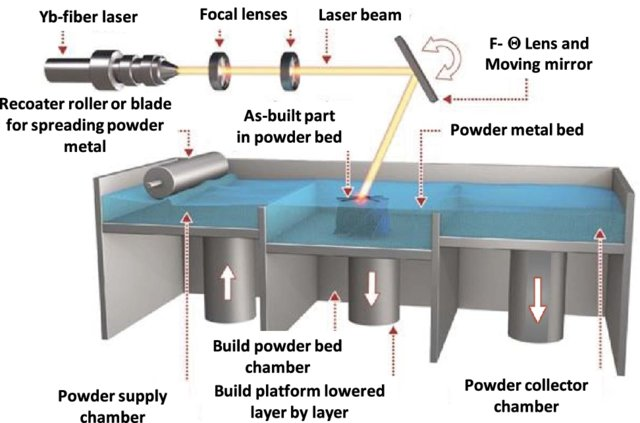
\includegraphics[scale=1.1]{Images/PBF.jpg}
    \caption[Laser PBF in AM.]{Laser powder bed fusion process in additive manufacturing. Adapted from \cite{ozel_focus_2020}.}
    \label{fig:PBF}
\end{figure}
The first operations in SLS printing are the calibration of the plate mounting and the formation of a vacuum atmosphere inside the printer chamber. Sometimes, a regular flow of inert gas is introduced to obtain controlled and uniform melting of the metal powder to minimize oxidation and degradation of the powdered material. Directing an inert gas is preferred to maintaining a vacuum atmosphere in an industrial context mainly for two reasons. First, maintaining a vacuum atmosphere throughout the printing process requires much effort. Second, reducing the pressure in the process chamber can lower the metal boiling point, leading to excessive smoke and vapor. The mixture of vaporized metal and smoke can affect the effectiveness of the laser as it is an optical device, and, as we all know, microparticles suspended in the air could deflect the laser beam. For the same reason, high reflective materials cannot be used, otherwise the laser energy would be lost in the printing chamber. Once the inert gas flow is established, the roller or the blade responsible for distributing the powder performs a rapid powder re-coating. Then, an electric resistor under the powder bed preheats the powder at a temperature of about \SI{500}{\degreeCelsius}. This operation helps to reduce the gap between the temperature of the chamber and the metal's melting point and also helps maintain a uniform temperature within the building bed. This is necessary to prevent the warping of the part during the printing due to non-uniform thermal expansion and contraction, which will lead to cracks and fractures (see Section \ref{sec:defects}). After these preliminary operations, the printing process can begin. A scanning system composed of a laser diode and a galvanometric mirrors system selectively melts the metal, alternating layer after layer with the powder distribution blade.  Laser equipment can generate powers in the range of thousands of watts and can focus to beam spot sizes of fractions of a millimeter. These small spot sizes have the potential to create minuscule molten pools, scanning the surface with a velocity of up to several meters per second. Nowadays, almost all lasers used in AM rely on active optical fiber sources. A schematic representation can be seen in Fig. \ref{fig:detailedfiber}. The energy transferred from the laser to the powder bed depends on the laser power (\numrange[range-phrase = --]{100}{1000}\unit{\watt}), the light-absorbing capacity of the material, and the scanning speed, which can be controlled (and it is limited) by the angular velocity of the galvanometer. The galvanometer system, Fig. \ref{fig:galvano}, consists primarily of two mirrors rotating along their axis, directing the laser beam to the desired point. The photon beam passes through a series of f-theta lenses that facilitate rapid laser movement and precise focusing of the laser spot. After completing the printing process, it is necessary to allow the object to cool down. Although supports are not always required, as the powder supports the object itself, they may need to ensure uniform heat transmission during the printing and cooling phase. Once the object has cooled down, we can remove any excess powder. The excess powder can be recycled and reused after undergoing preliminary processing and strict conformity controls, as each time it is reused, it loses some of its features \cite{strondl_characterization_2015}. Finally, post-processing operations, such as removing supports, surface finishing, and annealing, can be carried out if required. The latter is needed if the cooling phase inside the chamber has created an undesired microstructure in the final piece.
\begin{figure}
    \centering
    \subfloat[\label{fig:galvano}]{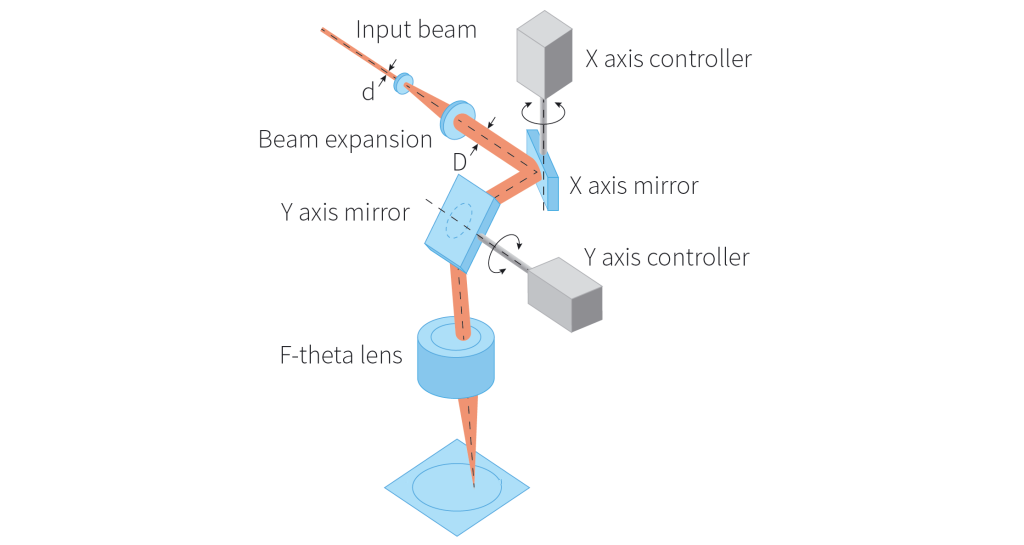
\includegraphics[scale=0.3]{Images/galvanometro.png}}
    \quad
    \subfloat[\label{fig:electrongun}]{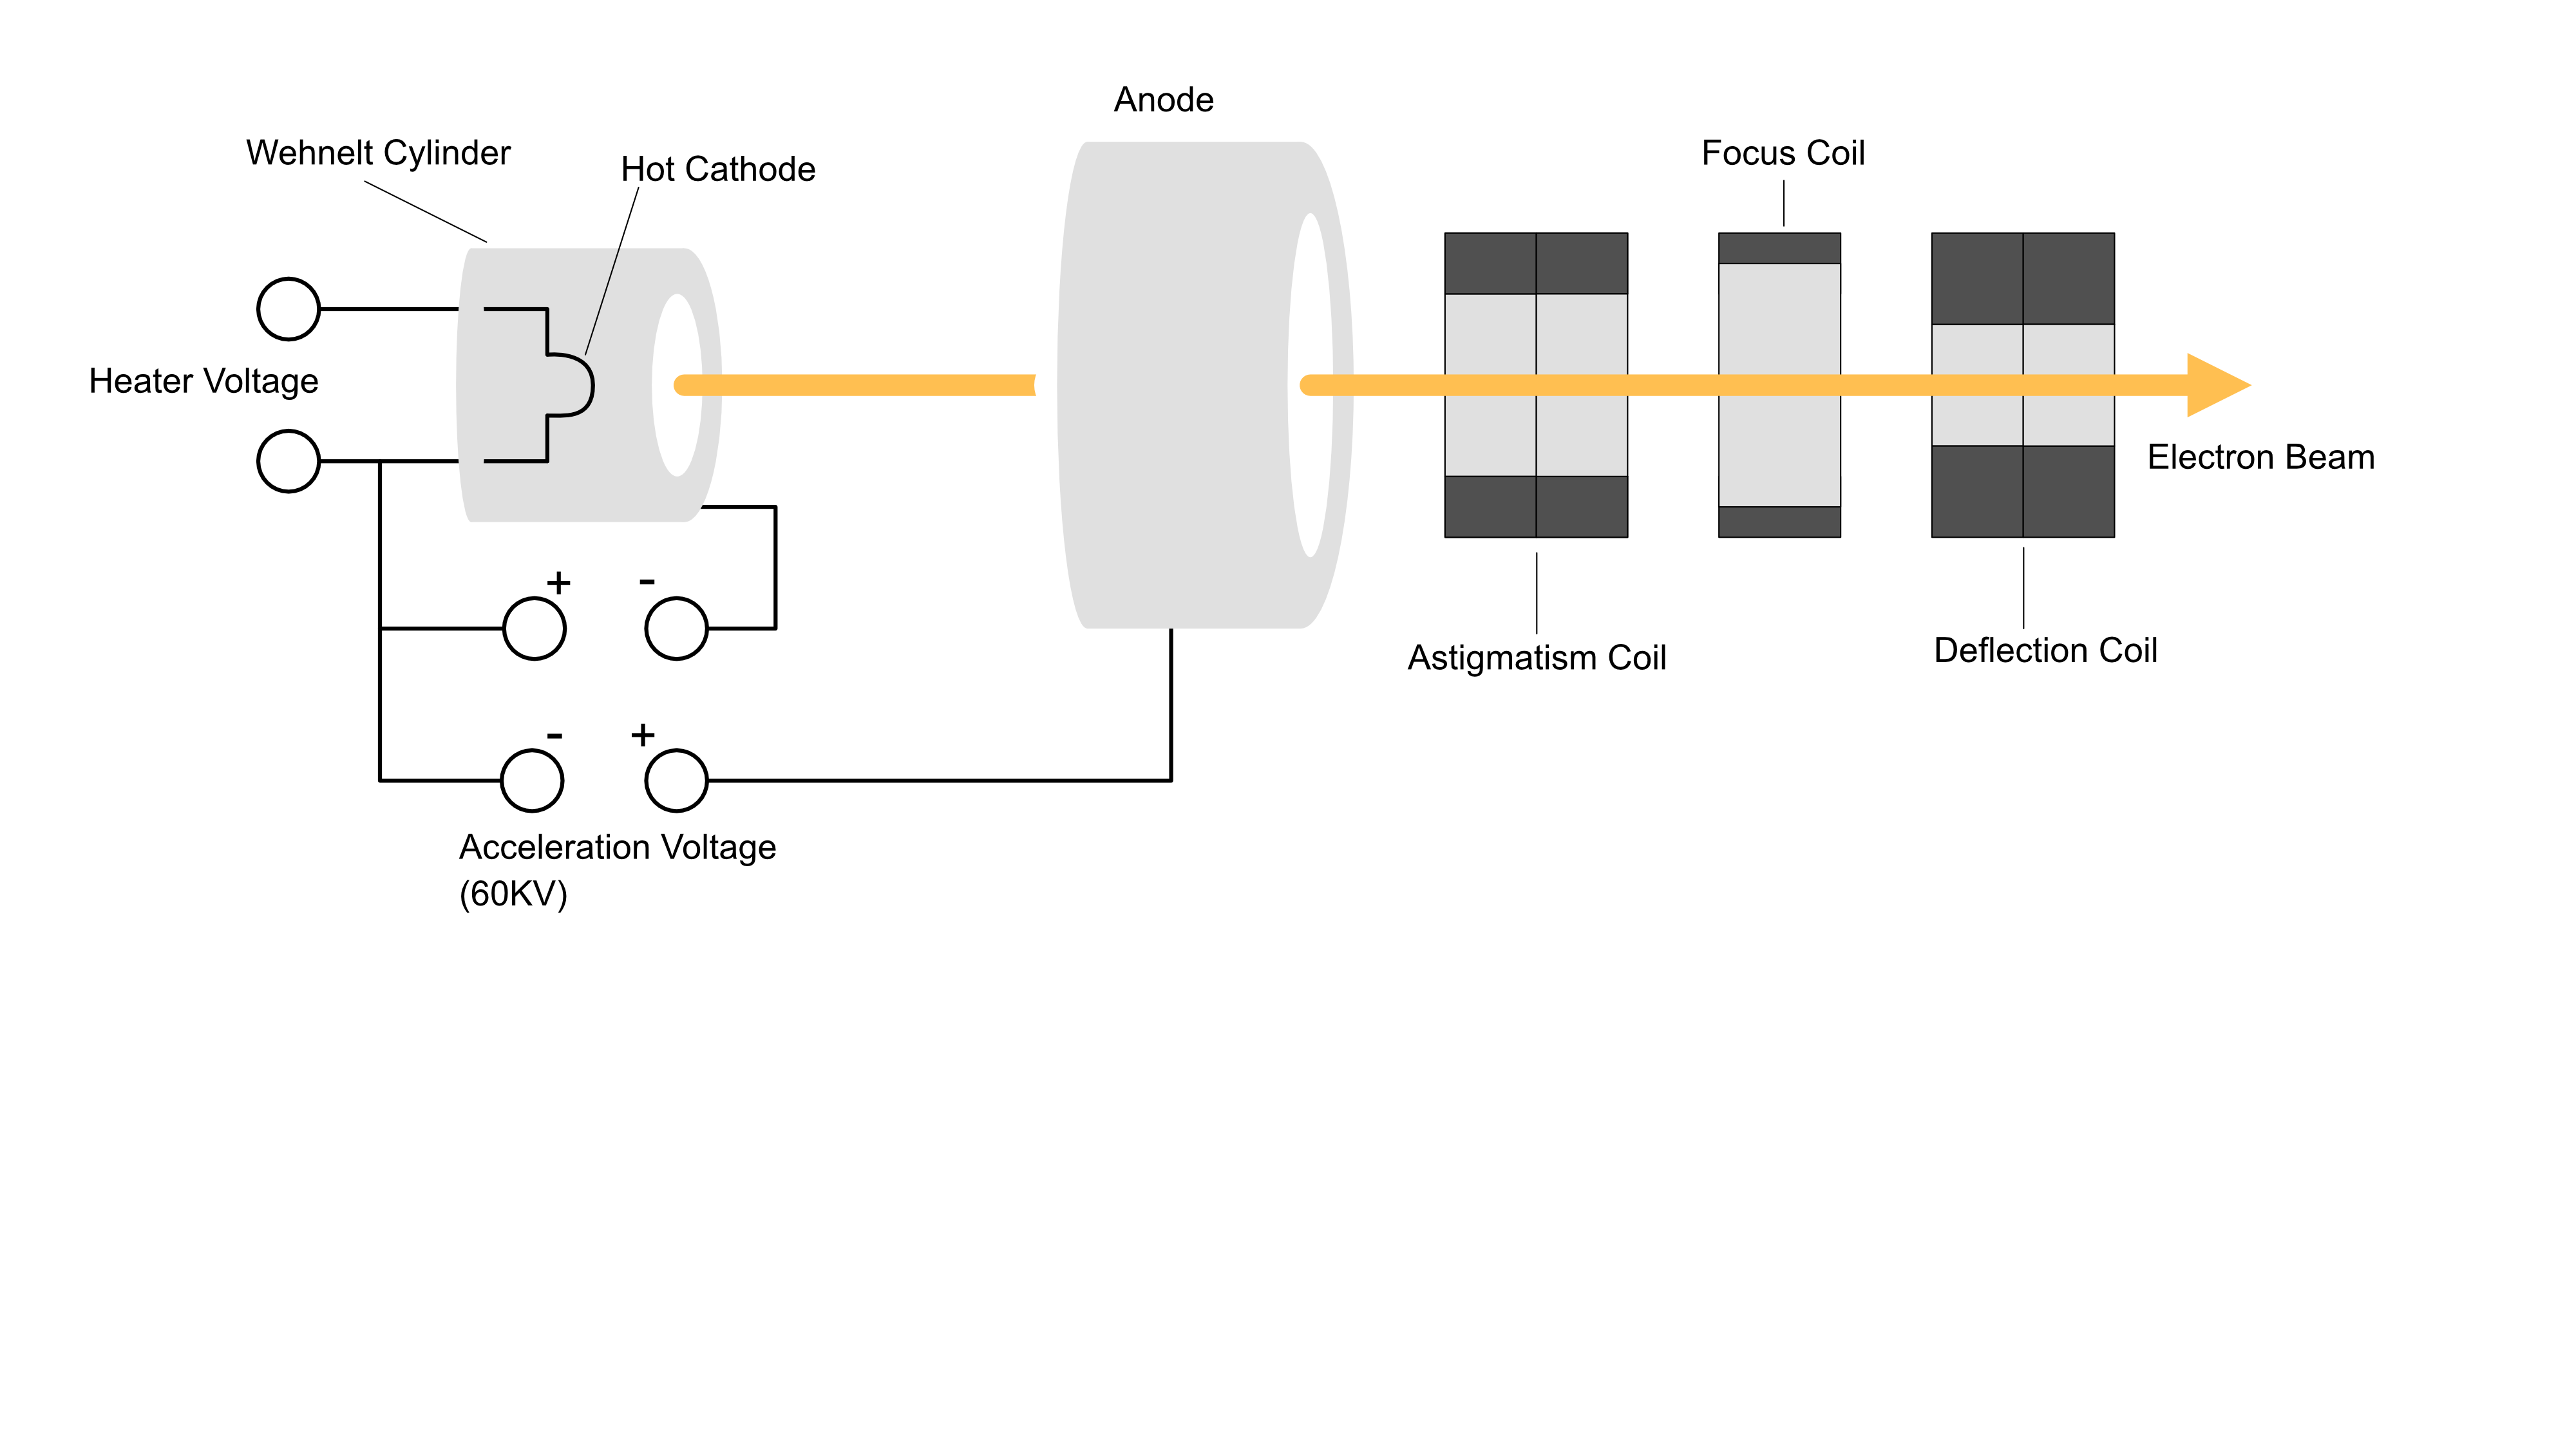
\includegraphics[width=0.7\textwidth]{Images/EBM.png}}
    \caption[Galvanometric system and electron gun.]{Dual-axis galvanometric system (a) and electron gun schema (b).}
\end{figure}
% <<<SLS

%%%%%
%%%%%

% EBM >>>
\subsection{Electron Beam Melting}
\label{subsec:ebm}
In EBM printers, the process is fundamentally the same as in laser printers. The metal powder is selectively melted, with a recoater blade providing additional metal powder after each layer. However, the energy source is not a laser (i.e., a beam of photons) but rather a beam of electrons generated by an electron gun. An electron gun is composed of a metallic filament, typically tungsten or tantalum, passed through by an electric current to produce an electron beam. The resulting electron beam is then directed through a Wehnelt cylinder. By negatively or positively charging the cylinder, we can block or allow the passage of electrons respectively. Fig. \ref{fig:electrongun} shows a diagram of the electron gun beam's structure. An anode charged with a voltage of up to \SI{60}{\kilo\volt} accelerates the electrons and directs the beam into the column through magnetic lenses. Unlike SLS printers, which rely on optical lenses, the lenses in EBM printers are magnetic. Section \ref{sssec:magneticlens} provides a more comprehensive description of magnetic lenses. EBM printers require a vacuum atmosphere inside the printing chamber to work correctly, and a minute amount of helium must be continuously injected into the chamber to prevent the accumulation of electric charges due to residual electrons on the powder bed. The phenomenon will be discussed in Section \ref{subsec:ebminter}. To put the "minuscule amount" of helium required into perspective, consider that the pressure in the vacuum atmosphere inside the chamber is \SI{0.05}{\pascal}, and the pressure with helium flow is about \SI{0,2}{\pascal} (recall atmospheric pressure is \SI{1,01325e5}{\pascal}). Another significant difference is the preheating phase. This stage does not occur through an electric resistor but rather through an initial electron beam scan that happens at two distinct moments. During the first phase, the entire powder bed is scanned, while only sub-regions of the powder bed that will be printed are scanned during the second phase. Preheating phases help avoid the so-called "smoke effect" caused mainly by the electrostatic repulsion in the powder. Furthermore, the preheating stage is necessary for obtaining final objects with better performance and reduces the need for support structures during printing. This allows for the use of the entire volume of the powder bed container when printing. 
\begin{figure}
    \centering
    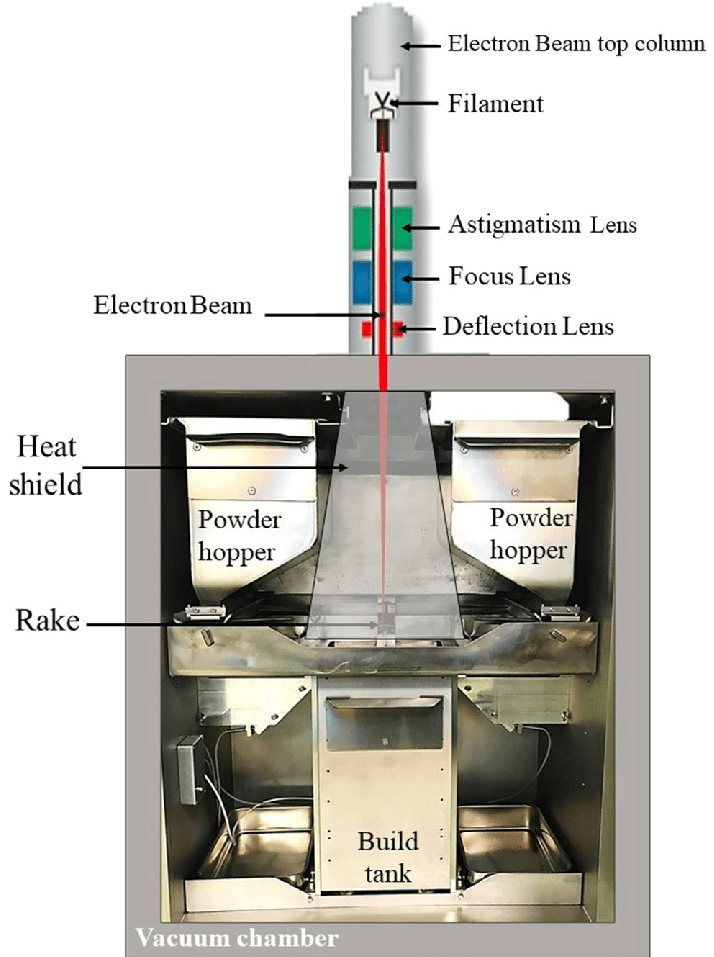
\includegraphics[scale=0.25]{Images/A-schematic-of-electron-beam-melting-EBM.png}
    \caption[EBM 3d-printer.]{Electron beam melting 3d-printer \cite{azam_-depth_2018}.}
    \label{fig:ebm_printer}
\end{figure} 
Thus, it is possible to print multiple objects, one on top of the other, since no support would interfere with them. However, this dual preheating phase causes the excess powder to solidify around printed pieces and must be removed with the same loose metal powder. Another structural difference of an EBM printer can be seen in Fig. \ref{fig:ebm_printer}. Due to the vacuum inside the print chamber and the consequent lowering of the metal's vaporization temperature, a heat shield is required around the chamber to prevent the vaporized metal from condensing and creating a film on the entire printer structure. The heat shield acts as a physical barrier, allowing easy removal and disposal of the metal film produced during printing.
\begin{table}
\small
    \centering 
    \begin{tabular}{|l l l|}
    \hline
    \rowcolor{bluepoli!40} % comment this line to remove the color
     & \textbf{EBM} & \textbf{SLS} \T\B \\
    \hline \hline
    \textbf{Energy source} & Electron beam & Laser  \T\B \\ 
    \textbf{Chamber atmosphere} & Vacuum(Almost) & Inert gas  \T\B\\
    \textbf{Scanning} & Magnetic lenses & Galvanometers \T\B \\
    \textbf{Energy absorption} & Conductivity-limited & Absorptivity-limited \T\B\\
    \textbf{Scan speeds} & Very fast & Limited by galvanometer inertia \T\B\\
    \textbf{Energy costs} & Moderate & High \T\B\\
    \textbf{Feature resolution} & \numrange{100}{200}\unit{\micro\metre} & \numrange{75}{100}\unit{\micro\metre}  \T\B\\
    \textbf{Materials} & Conductors & Polymers, metals and ceramic \T\B\\
    \textbf{Layer Thickness} & \SI{50}{\micro\metre} & \SIrange{10}{50}{\micro\metre}  \T\B\\
    \textbf{Min Wall Thickness} & \SI{0.6}{\milli\metre} & \SI{0.2}{\milli\metre} \T\B\\
    \textbf{Accuracy} & $\pm$\SI{0.4}{\milli\metre} & $\pm$\SI{0.3}{\milli\metre} \T\B\\
    \textbf{Build rate} & \numrange[range-phrase=--]{55}{80}\unit{\centi\metre^3 / \hour} & \numrange[range-phrase=--]{60}{100}\unit{\centi\metre^3 / \hour} \T\B\\
    \textbf{Powder Particle Size} & \numrange[range-phrase = --]{40}{105}\unit{\micro\meter} & \numrange[range-phrase = --]{15}{45}\unit{\micro\meter} \T\B\\
    \hline
    \end{tabular}
    \\[10pt]
    \caption{Comparison between SLS and EBM processes. Adapted from \cite{gallina_electron_2017}.}
    \label{table:slsvsebm}
\end{table}
There are also differences in the materials used for printing. In EBM printing, usually metal powder size is slightly larger than the powder used in laser printing, with a particle size of approximately \numrange[range-phrase = --]{40}{105}\unit{\micro\meter} against the \numrange[range-phrase = --]{15}{45}\unit{\micro\meter} in SLS processes. Furthermore, the metal powder must exhibit good electrical conductivity. Indeed, electrons penetrate the matter thanks to the material's electrical conductivity, making inert materials unsuitable for this printing process. On the other hand, with EBM, we can also use reflective materials, as mirrored surfaces do not repel electrons. 
Table ~\ref{table:slsvsebm} highlights the main differences between the two processes described in previous sections.
% <<< End of EBM

%%%%%
%%%%%

% Metal Powders >>>
\section{Metal Powders for AM} 
\label{sec:metalpowders}
As seen in Section \ref{sec:pbf_proc}, PBF processes require metal powders. Various metallic materials can be transformed into powders suitable for additive manufacturing to be used in different sectors according to their mechanical properties. Table \ref{table:materialAMmetal} shows some examples of metallic materials currently available on the market and the respective industrial sectors in which they are used. In most cases, these powders are produced using atomization processes that exploit various physical methods to generate micro-particles. The resulting particles are characterized by a more or less spherical shape and a certain chemical purity that depend on the method used to produce them. The inefficiency and cost of atomization processes used is the reason why, in the case of specific high-quality powders, the powder price can be up to 10 times the cost of the raw metal. \citeauthor{deng_origin_2020} (2020) have demonstrated that powders made of irregular micro-particles and with low chemical purity can lead to structural defects in the final parts, resulting in lower performance. Therefore, over the years, increasingly complex and expensive processes have been developed to obtain higher-quality powders.
\begin{table}
\centering 
\small
    \begin{tabular}{|l l l|}
    \hline
    \rowcolor{bluepoli!40}
    \textbf{Material} & \textbf{Examples} & \textbf{Applications}\\
    \hline \hline
    \textbf{Stainless steel} & 316L, 174-PH, MS1, M300 & Food, biomedical, consumer \T\B\\
    \textbf{Ni-alloys} & In625, In718, In939 & Energy, motorsport\T\B\\
    \textbf{Al-alloys} & AlSi12, AlSi10Mg & Lightweight, aerospace, aviation\T\B\\
    \textbf{CoCr-alloys} & CoCrMo & Dental, biomedical\T\B\\
    \textbf{Ti-alloys} & Ti6Al4V, CP Ti & Biomedical, lightweight, aerospace\T\B\\
    \textbf{Tool steel} & Maraging 18Ni300 & Tooling, aerospace, automotive\T\B\\
    \textbf{Cu-alloys} & Bronze & Energy, heat exchanger\T\B\\
    \textbf{Precious} & Au, Pt, Ag & Jewellery, design\T\B\\
    \hline
    \end{tabular}
    \\[10pt]
    \caption{Material availability for metal AM.}
    \label{table:materialAMmetal}
\end{table}
\begin{figure}
    \centering
    \subfloat[\label{fig:wateratom}]{
        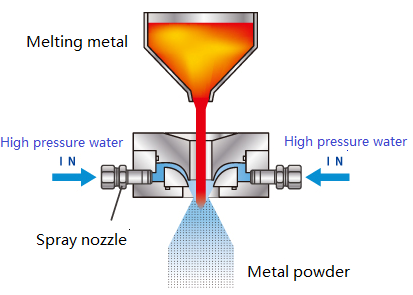
\includegraphics[scale=0.45]{Images/wateratom.png}
    }
    \qquad
    \subfloat[\label{fig:gasatom}]{
        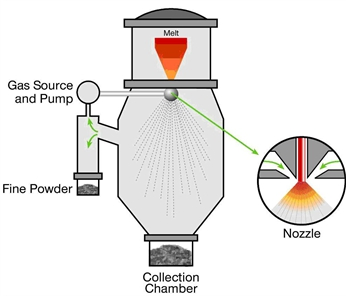
\includegraphics[scale=0.45]{Images/gasatom.png}
    }
    \\
     \subfloat[\label{fig:plasmaatom}]{
        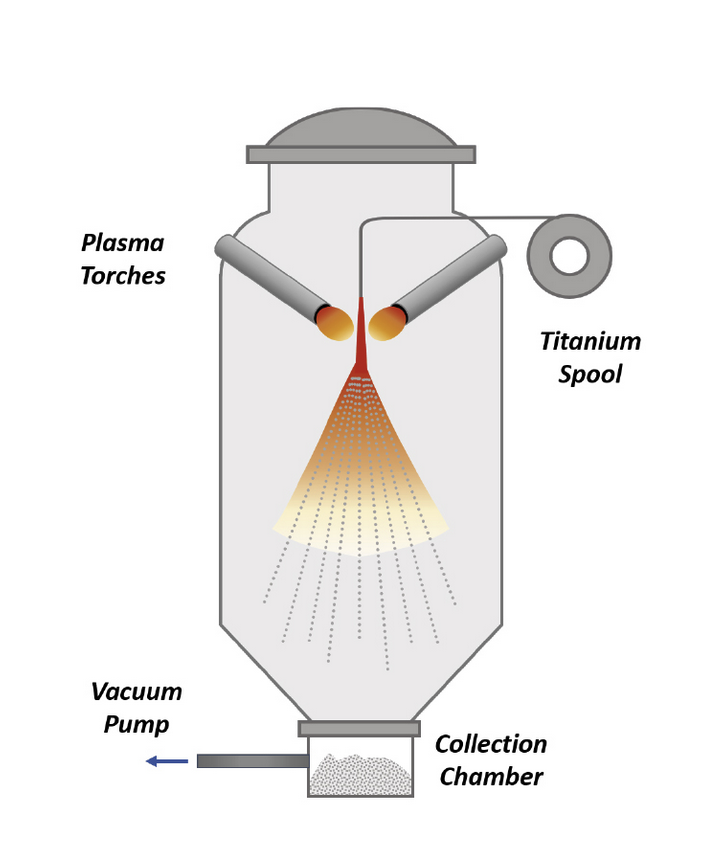
\includegraphics[scale=0.28]{Images/plasma.png}
    }
    \qquad
    \subfloat[\label{fig:repatom}]{
        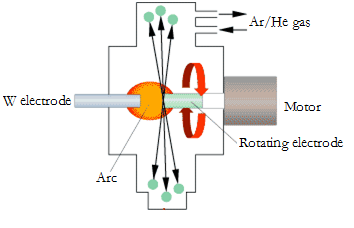
\includegraphics[scale=0.53]{Images/repatom.png}
    }
    \caption[Atomization processes.]{Water atomization process (a), gas atomization process (b), plasma atomization process (c) and rotating electrode process (d) \cite{material_technology_innovations_co_rotating_2020, material_technology_innovations_co_water_2020, material_technology_innovations_co_gas_2020, inovar_communications_ltd_metal_2020}.}
    \label{fig:atom}
\end{figure}
\paragraph{Water atomization.}The process of water atomization of metals, Fig. \ref{fig:wateratom}, involves the production of tiny droplets by exposing a stream of molten metal to a high-pressure jet of water. The water atomization process is typically carried out in a chamber where the molten metal is injected into a nozzle that directs the stream of liquid metal toward a high-pressure jet of water. As the molten metal comes into contact with the water, it rapidly cools down and solidifies, forming tiny droplets collected at the bottom of the chamber. The size and shape of the particles obtained during the water atomization process can be controlled by adjusting the temperature of the molten metal, the pressure of the water jet, and the distance between the nozzle and the water jet. By handling these parameters, it is possible to produce metal powders with a range of particle sizes between \numrange[range-phrase = --]{1}{500} \unit{\micro\metre}. The output-to-input ratio for this process is approximately 95\%, which means that from \SI{1}{\kilo\gram} of raw metal, it is possible to obtain up to \SI{950}{\gram} of powder. Compared to other powder production methods, the water atomization process offers several advantages, including high production rates, the wide range of particle sizes obtainable, and metal ingots can be used as process input, shortening this production process's manufacturing chain. It is also characterized by a higher output-to-input ratio. On the other hand, the process leads to a low chemical purity and irregular particle shapes, as in Fig. \ref{fig:waterpow}, and needs extensive post-processing operations to obtain a decent-quality product. Moreover, it cannot be used with reactive materials such as titanium and aluminum.
\paragraph{Gas atomization.} The process of gas atomization, Fig. \ref{fig:gasatom}, can be performed using a variety of gases, depending on processed metals. The most commonly used gases are inert gases such as nitrogen, argon, and helium, even if the latter is barely used in industrial applications due to its high cost. Inert gases are preferred because they do not react with the molten metal and do not introduce impurities into metal particles. Metal ingots are molten, and the flow is rapidly solidified by exposing it to a high-pressure gas stream. The main advantages are its high production rate, a wide range of obtainable particle sizes, applicability to reactive materials, and ability to ensure good chemical purity. The main drawbacks are mostly related to the porosity of the resulting powder and the formation of small satellite particles.
\begin{figure}
    \centering
    \subfloat[\label{fig:waterpow}]{
        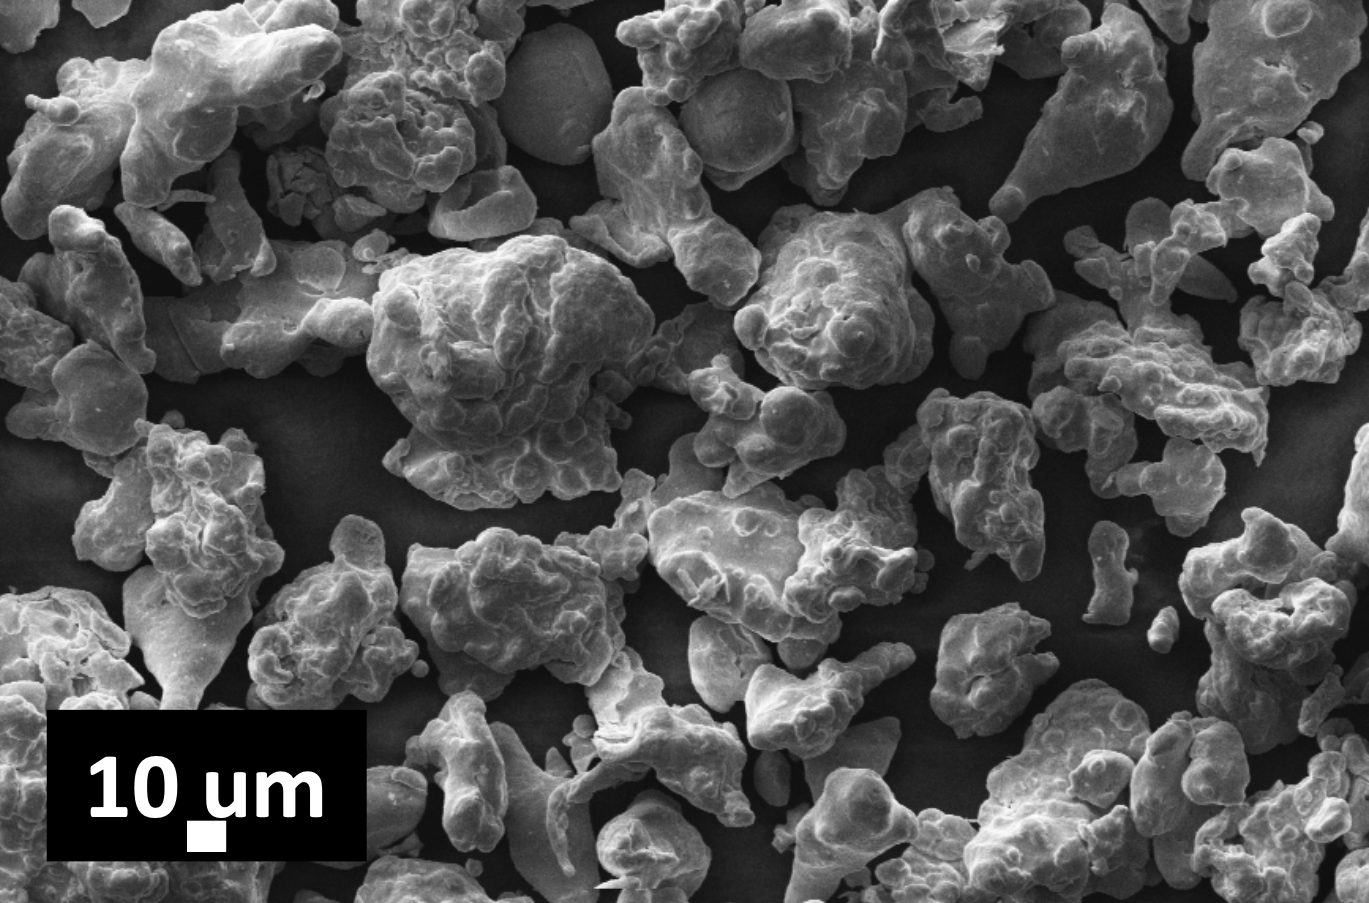
\includegraphics[scale=0.22]{Images/waterpow.png}
    }
    \qquad
    \subfloat[\label{fig:gaspow}]{
        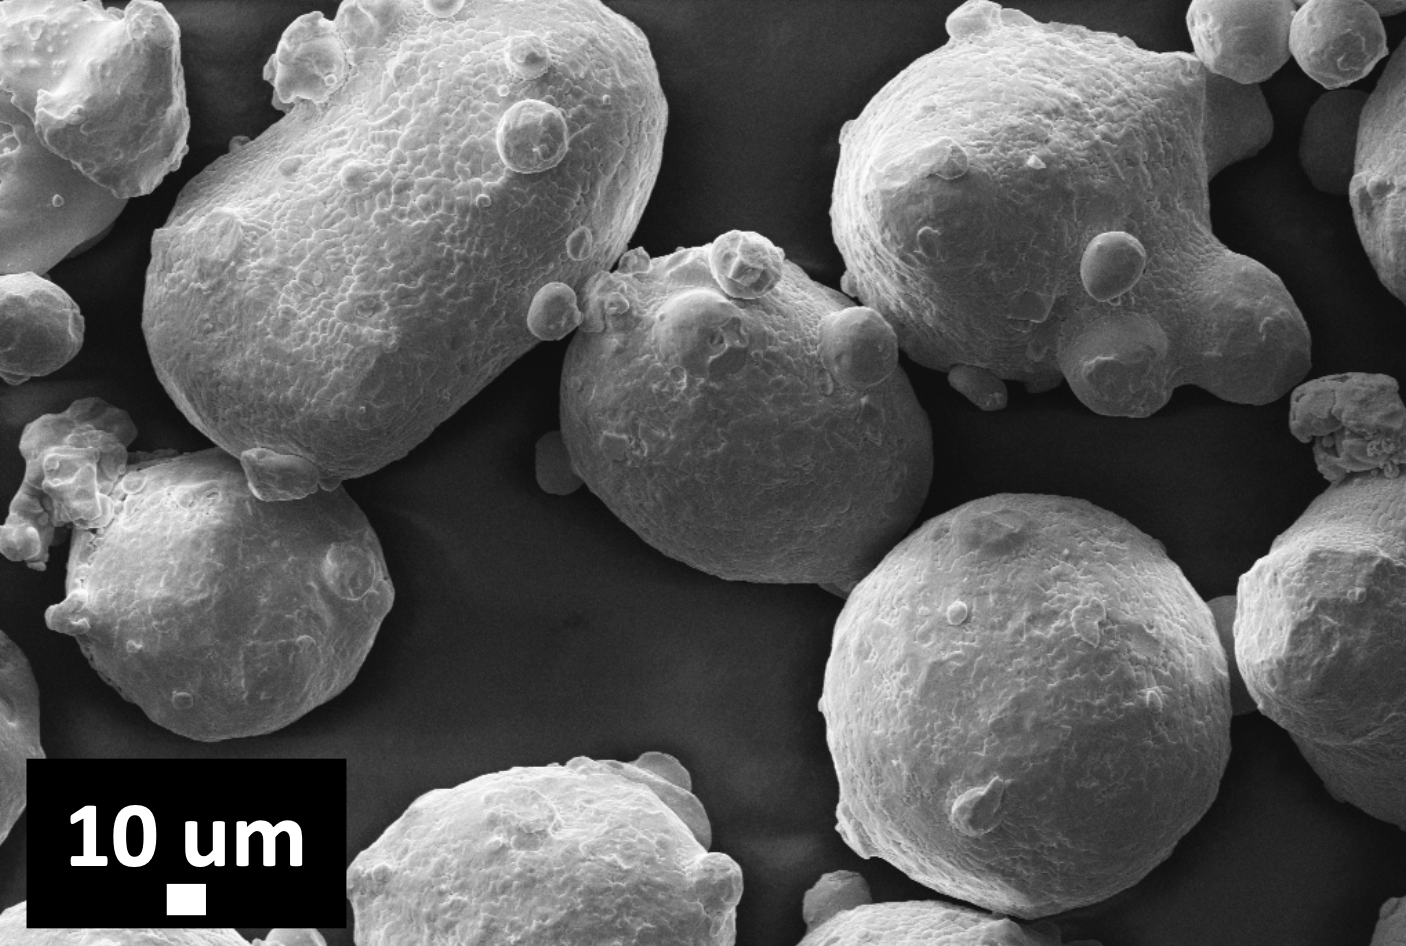
\includegraphics[scale=0.21]{Images/gaspowd.png}
    }
    \qquad
     \subfloat[\label{fig:plasmapow}]{
        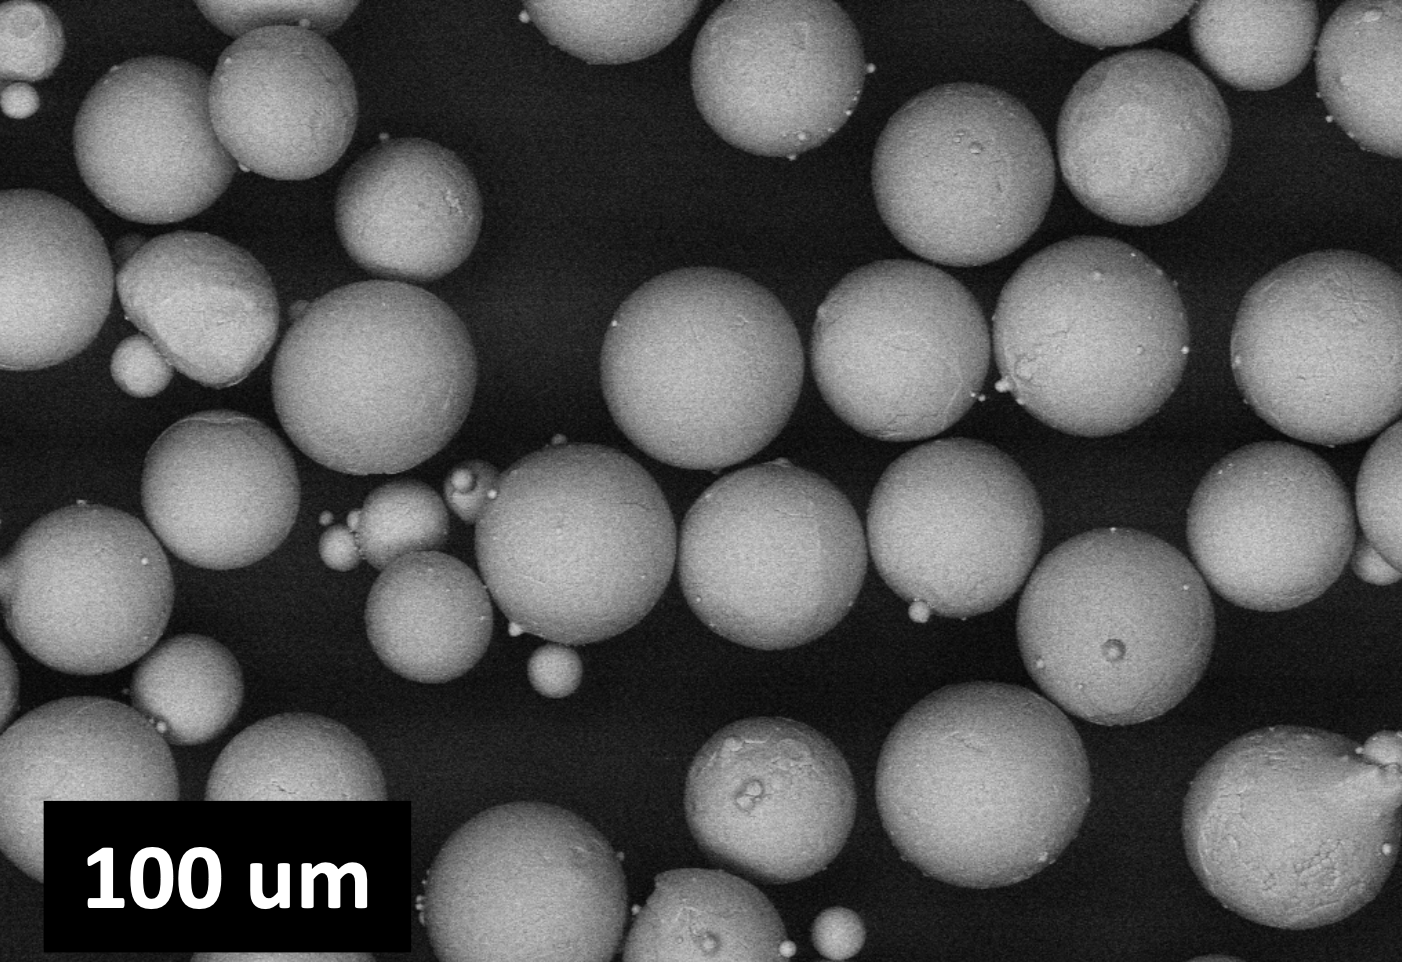
\includegraphics[scale=0.22]{Images/plasmapowder.png}
    }
    \qquad
    \subfloat[\label{fig:reppow}]{
        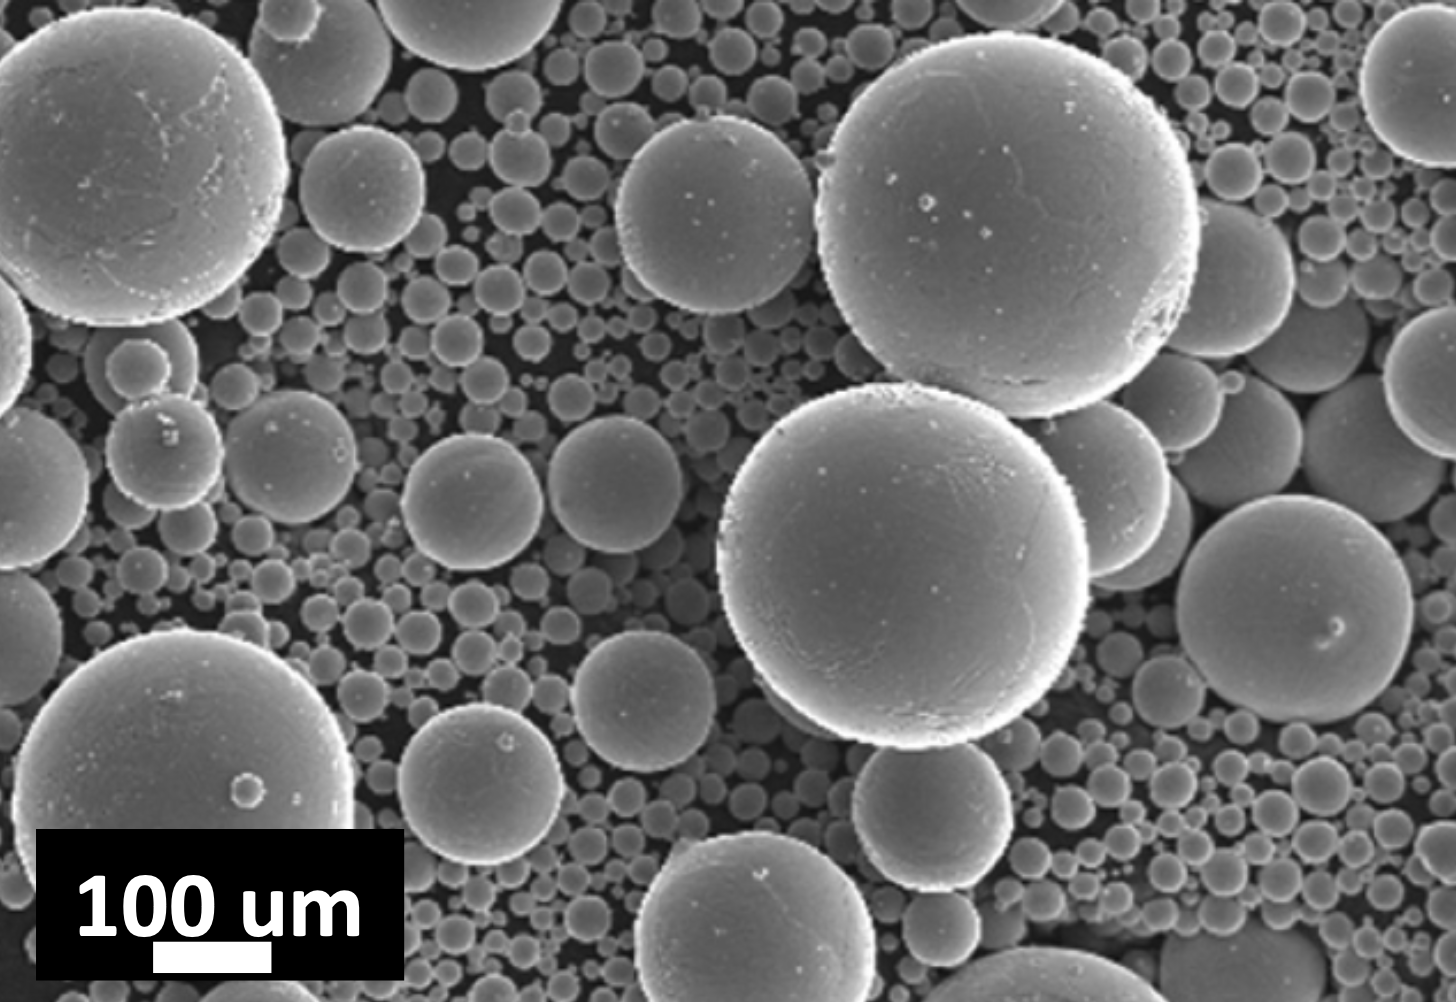
\includegraphics[scale=0.21]{Images/erppowder.png}
    }
    
    \caption[Powders obtained from atomization processes.]{Micro-particles obtained by water atomization (a), gas atomization (b), plasma atomization (c) and rotating electrode process (d) \cite{slotwinski_characterization_2014}.}
    \label{fig:powders}
\end{figure}
\paragraph{Plasma atomization.} The plasma atomization process, Fig. \ref{fig:wateratom}, involves using high-temperature plasma torches to melt the metal wire. We can generate a high-energy plasma using an electric current through a non-consumable tungsten electrode and an inert gas jet to direct the welding arc into a focused area. As the molten metal droplets are expelled from the plasma jet, they rapidly solidify, sometimes also thanks to the water-cooled chamber, and break up into small, spherical particles, which are then collected in a container. The plasma atomization process offers several advantages over other powder production methods, including the ability to produce highly spherical-shaped particles. Moreover, it can be used with reactive material. Plasma atomization can also produce powders with very high purity levels since the plasma jet's high temperature helps eliminate impurities. However, it is more expensive than other powder production methods due to the need for specialized equipment and the high energy consumption required to generate the plasma arc. The process can also be challenging to control, as parameter variations can highly impact the resulting particles' size, shape, and purity. Powders produced using this method have a low size range of about \numrange[range-phrase = --]{1}{200}\unit{\micro\metre}.
\paragraph{Rotating electrode process.} In the rotating electrode process, Fig. \ref{fig:repatom}, a consumable metal electrode is rotated at high speeds. At the same time, an electric arc melts it in a chamber with a continuous inert gas flow. As the molten metal is exposed to the high-velocity inert gas stream, it rapidly solidifies and breaks into small droplets collected at the bottom of the atomization chamber. Due to its very high cost, this production method is typically used for metal powders with a perfectly spherical shape and without any impurities, e.g., gold. Fig. \ref{fig:reppow} shows the potential of this technology in obtaining perfect spherical micro-particles.
% <<< End of Materials

%%%%%
%%%%%

% Energy matter interactions >>>
\section{Energy - Matter Interactions}
\label{sec:matterint}
This section should be regarded as "optional", and it is up to the reader's discretion whether to engage with it. This section delves deeply into the physical processes underlying the technologies previously discussed. As said, in SLS, there is an interaction between photons and metal powder, while in EBM, there is an interaction between electrons and metal powder.
\subsection{Laser - Matter Interaction}
\label{subsec:sintering}
LASER is an acronym that stands for "light amplification by stimulated emission of radiation," and it is a monochromatic beam of photons characterized by low divergence and a focal spot size of \numrange[range-phrase = --]{30}{80}\unit{\micro\metre}. The type and color of the laser are two essential features of SLS. Indeed, the energy transmitted to the material depends on the energy absorption characteristics of the material that vary according to the wavelength of the laser source. For a successful fusion process, metallic powder particles must receive enough energy to melt.
\begin{figure}
    \centering
    \subfloat[\label{fig:laserintera}]{
        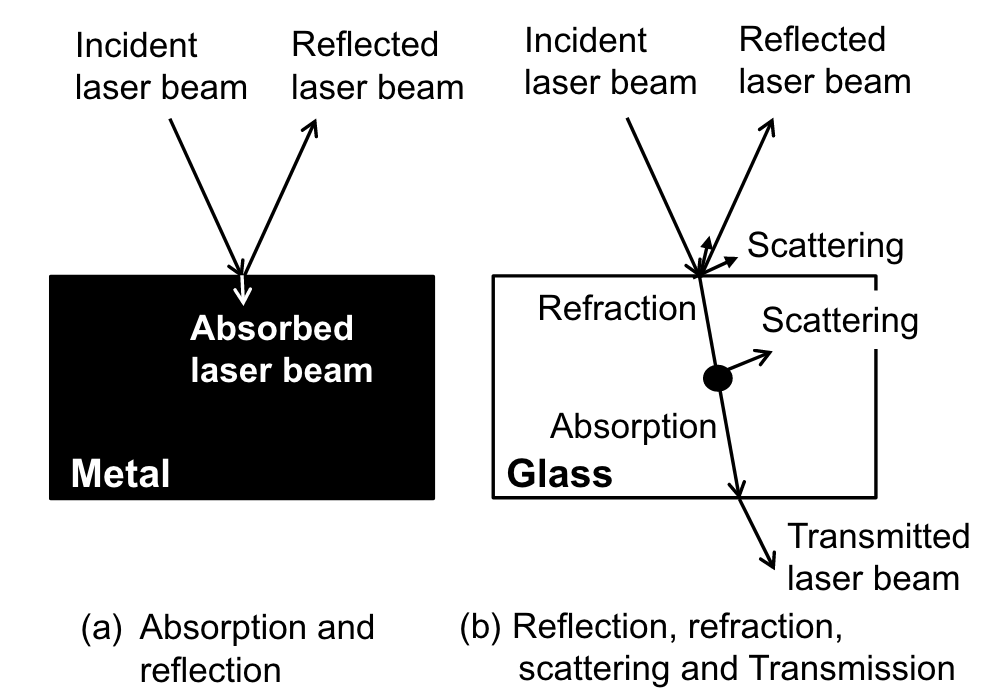
\includegraphics[scale=0.33]{Images/laser interactions.png}
    }
    \qquad
    \subfloat[\label{fig:laserintensity}]{
        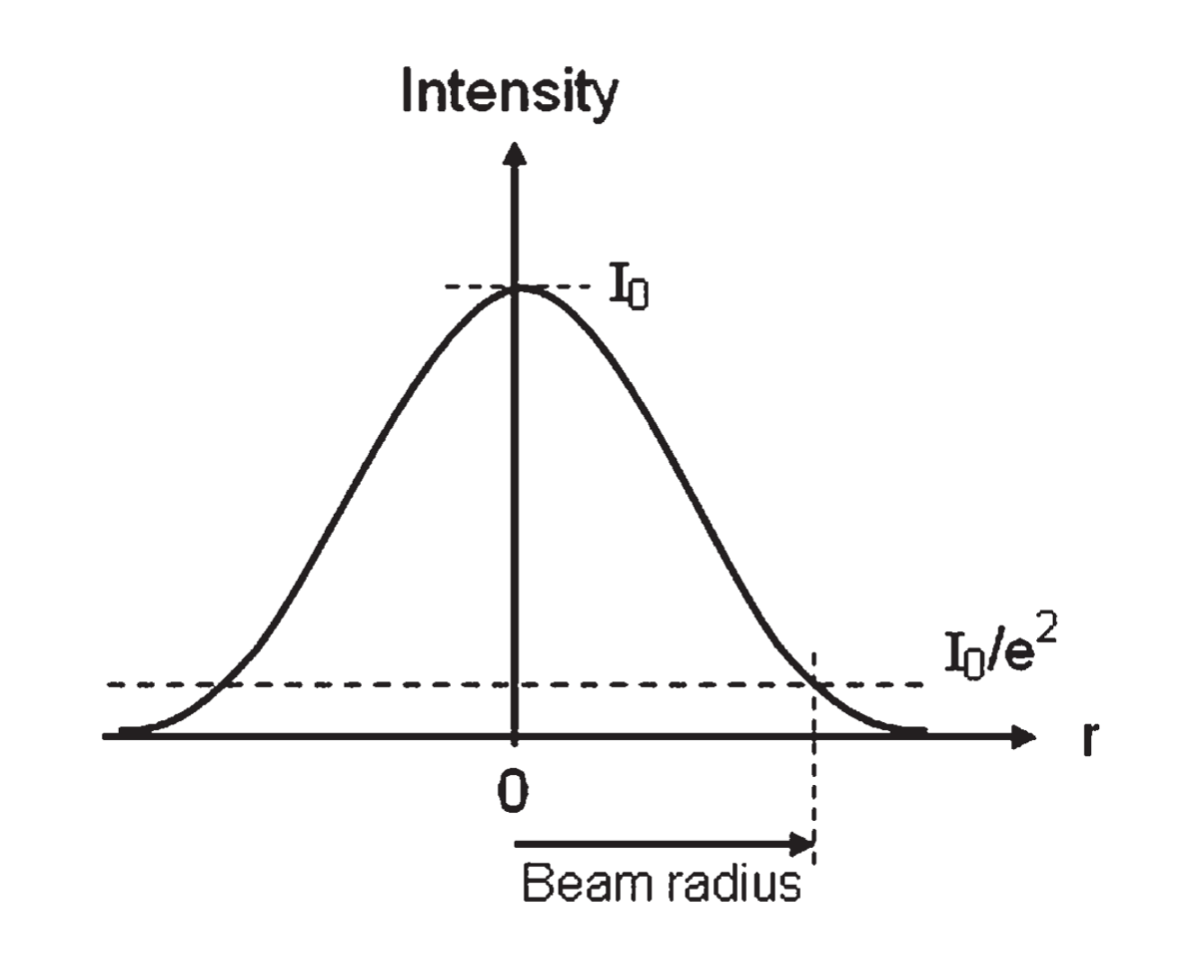
\includegraphics[scale=0.28]{Images/laserintensity.png}
    }
    
    \caption[Laser interactions and laser intensity.]{Schematic representation of physical interaction of absorption, reflection, transmission, refraction, and scattering between laser beam and material (a) \cite{katayama_fundamentals_2020}, and laser intensity schema (b).}
\end{figure}
For example, copper's absorptivity is about 50\% and 58\% for green and blue lasers, respectively, while it is just above 30\% for red lasers. In other words, green and blue lasers are more advantageous in processing copper powder in terms of higher initial absorption than other laser typologies. As we will explore later, the electron beam transfers energy to the material through charge movement. In contrast, the laser beam operates as an optical device, and hence, it is more sensitive to the behaviors illustrated in Fig. \ref{fig:laserintera}. Indeed, the metal specimen is highly reflective and opaque. This is also why the electron beam penetrates deeper into the metallic powder than the laser beam. The intensity of the laser emission varies as a function of the radius as 
\begin{equation}
    \label{eq:intensitylaser}
    I(r)=I_0\cdot e^{-2 \frac{r^2}{r_0^2}}
\end{equation}
Fig. \ref{fig:laserintensity} shows a schematic representation of density
The equation describes the energy density of the laser beam
\begin{equation}
    \label{eq:energydensity}
    E_d = \frac{P}{h\cdot v \cdot d}
\end{equation}
where $E_d$ is the energy density (\unit{\joule/\milli\metre^3}), $P$ is the laser power (\unit{\watt}), $v$ is the laser scan speed (\unit{\milli\metre / \second}), $h$ is the hatch distance (\unit{\milli\metre}), $d$ is the layer thickness of the powder(\unit{\milli\metre}). For a more detailed description of heat transfer, please refer to the next section. The intensity of the laser beam's energy plays a crucial role in SLS because if it is not correctly calibrated, the final piece might exhibit porosities that compromise its mechanical features. Another critical parameter to consider during the SLS process is the duration of the laser pulse. As shown in Fig. \ref{fig:pulsations}, a prolonged laser pulse results in a broad heat zone, causing a shock wave that leads to an increased debris formation during the interaction that can interfere with new layers.
\begin{figure}
    \centering
    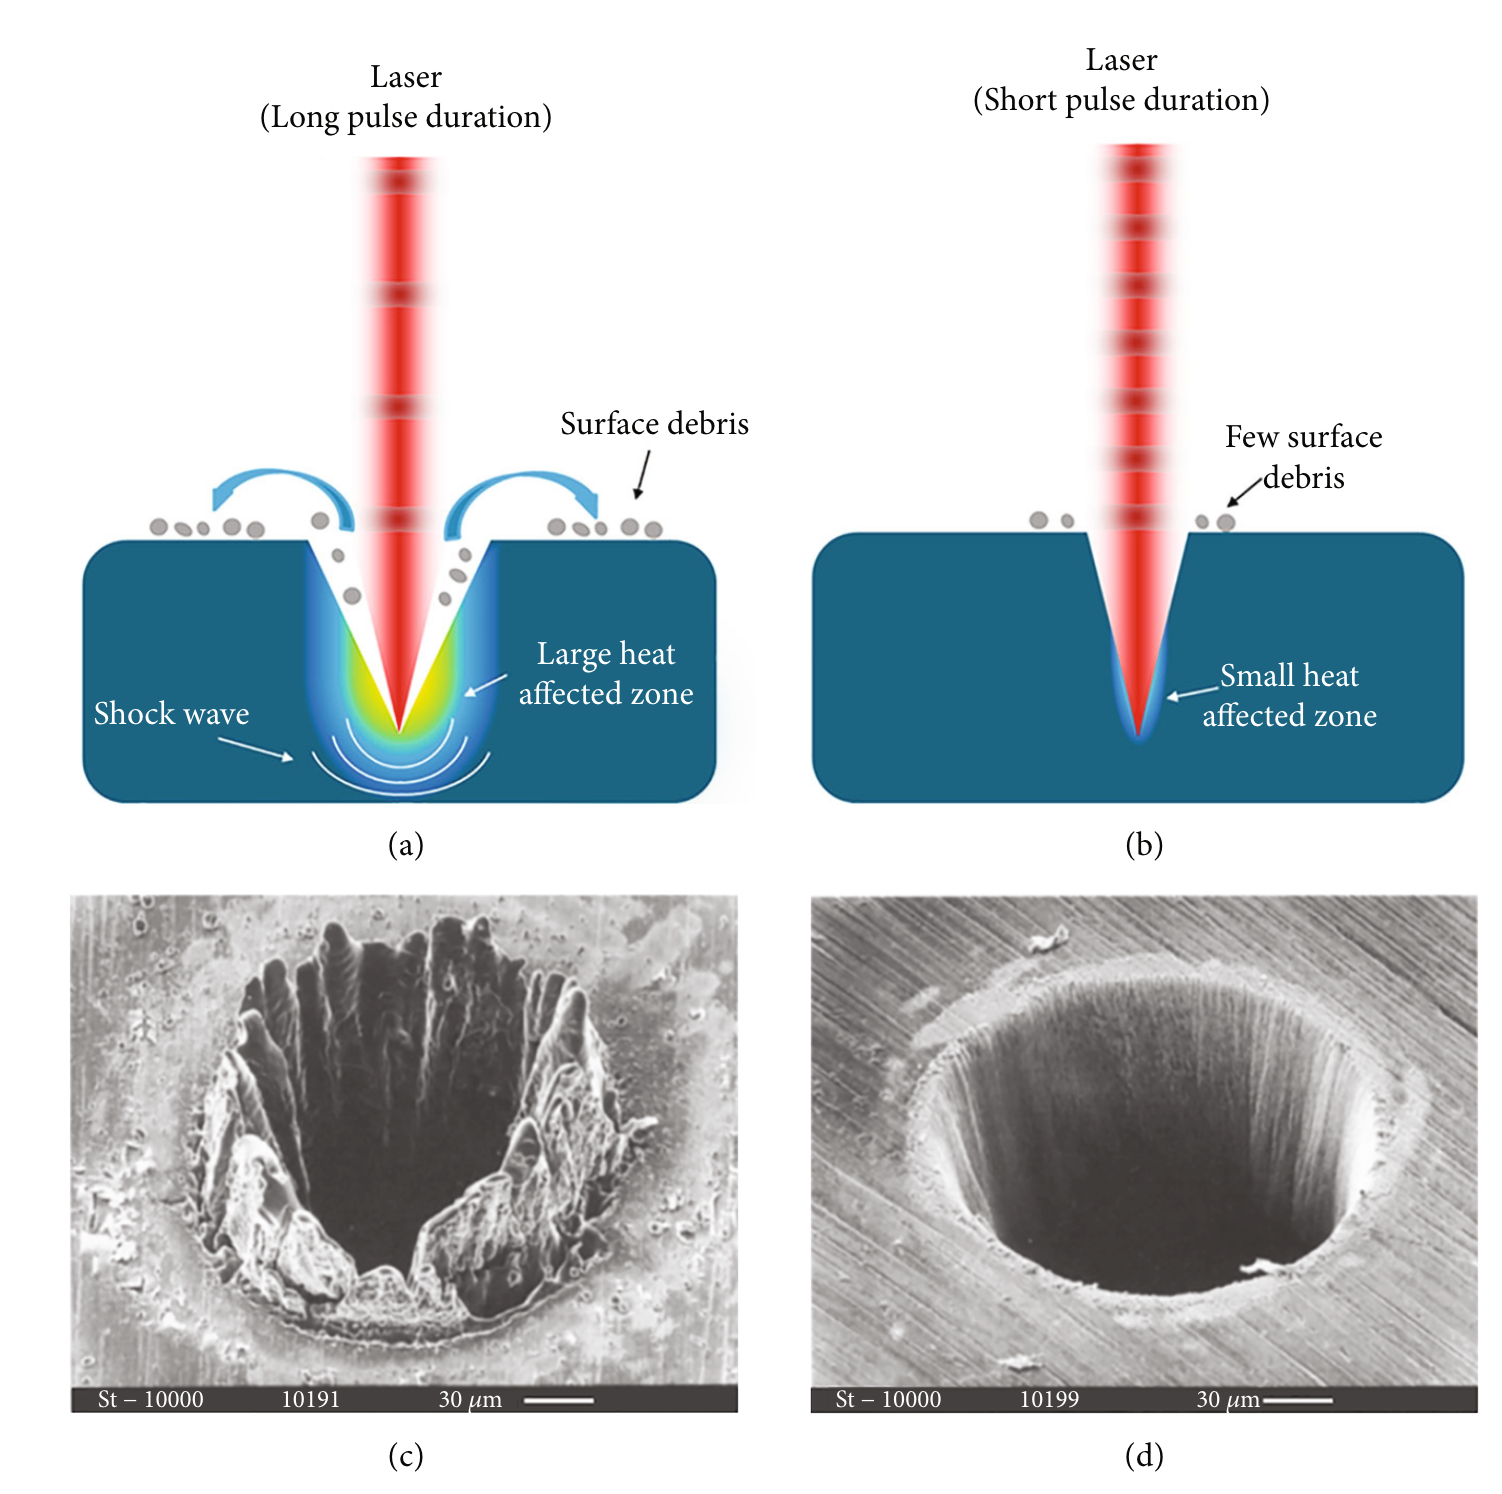
\includegraphics[scale=0.35]{Images/laserpulsing.png}
    \caption[Laser interactions with different pulses.]{Schematic of laser interaction with materials under different pulse duration: (a) long pulse duration and (b) short pulse duration and respective holes fabricated on a steel foil by (c-d) \cite{lin_femtosecond_2021}.}
    \label{fig:pulsations}
\end{figure}
For this reason, there has been a shift towards using ultra-short pulse lasers in recent years. These lasers are called "femtosecond lasers". They are also employed in precision processing or correction of semiconductors and liquid crystals, processing of transparent materials like glasses and sapphires, production of waveguide tubes for optical communication, and drilling of engine components for cars and aircraft, among other applications \cite{katayama_fundamentals_2020}. The high-frequency pulsation is achieved using a pulse stretcher, an amplifier, and a pulse compressor.
\subsubsection{Heat transfer}
\label{sssec:heattransfer}
Heat and mass movement influence heat and mass-related events in SLS. Laser heating is extremely rapid due to the fast scanning of laser velocities. In a closed system, with respect to the first law of thermodynamics, the energy balance equation is formulated as follows \cite{bouabbou_understanding_2022}:
\begin{equation}
    \label{eq:tutteQ}
    Q_L = Q_C + Q_{CV} + Q_R,
\end{equation}
where $Q_L$, $Q_C$, $Q_{CV}$, and $Q_R$ are the laser heat flux quantity, conduction, convection, and radiation heat quantities. Recalling that only $Q_C$ will contribute to the melting process. Thus, some of the energy applied to the powder bed will be lost in the form of heat convection and radiation. \\
To describe the heat conduction, we can use Fourier's law:
\begin{equation}
    \frac{\delta}{\delta x}\left(k \frac{\delta T}{\delta x}\right)+\frac{\delta}{\delta y}\left(k \frac{\delta T}{\delta y}\right)+\frac{\delta}{\delta z}\left(k \frac{\delta T}{\delta z}\right)+\dot{q} =\rho C_p \frac{\delta T}{\delta t}
\end{equation}
where $T$ (\unit{\kelvin}) is the temperature, $k$ (\unit{\watt.\metre^{-1}.\kelvin^{-1}}) is the thermal conductivity, $\dot{q}$ (\unit{\watt.\metre^{-3}}) is the rate of which the heat is applied to the system, $r$ (\unit{\kilo\gram.\metre^{-3}}) is the material density, $C_p$ (\unit{\joule. \kilo\gram^{-1}.\kelvin^{-1}}) is the specific heat and $t$ (\unit{\second}) is the interaction time between laser beam and powder particles.

\subsubsection{Optical Fiber Laser}
\label{sssec:fiberlaser}
One of the most common types of lasers used in SLS is the optical fiber laser \cite{milewski_additive_2017}, which relies on the light emitted by diodes. A diode is a semiconductor component acting like an unidirectional electric current gate. It allows the current to pass effortlessly in one direction but significantly hinders its flow in the opposite direction. Diodes have a polarity characterized by its anode (positive terminal) and cathode (negative terminal). Typically, diodes conduct current only when a positive voltage is supplied to the anode. In a laser diode (LD), an electric current is channeled directly through a dual hetero-junction structured semiconductor from the external side. When electrons recombine with positive holes at the active layer located between the n-type and p-type semiconductor zones, as shown in Fig. \ref{fig:np}, a light beam is emitted.
\begin{figure}
    \centering
    \subfloat[\label{fig:np}]{
        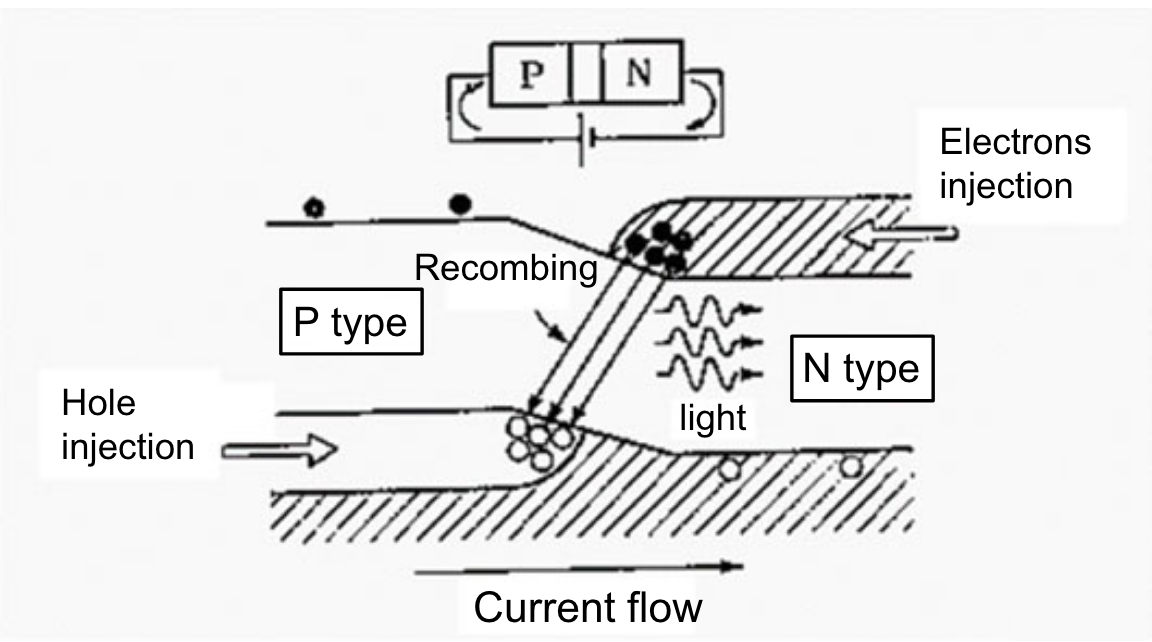
\includegraphics[scale=0.3]{Images/np.png}}
    \qquad
    \subfloat[\label{fig:detailedfiber}]{
        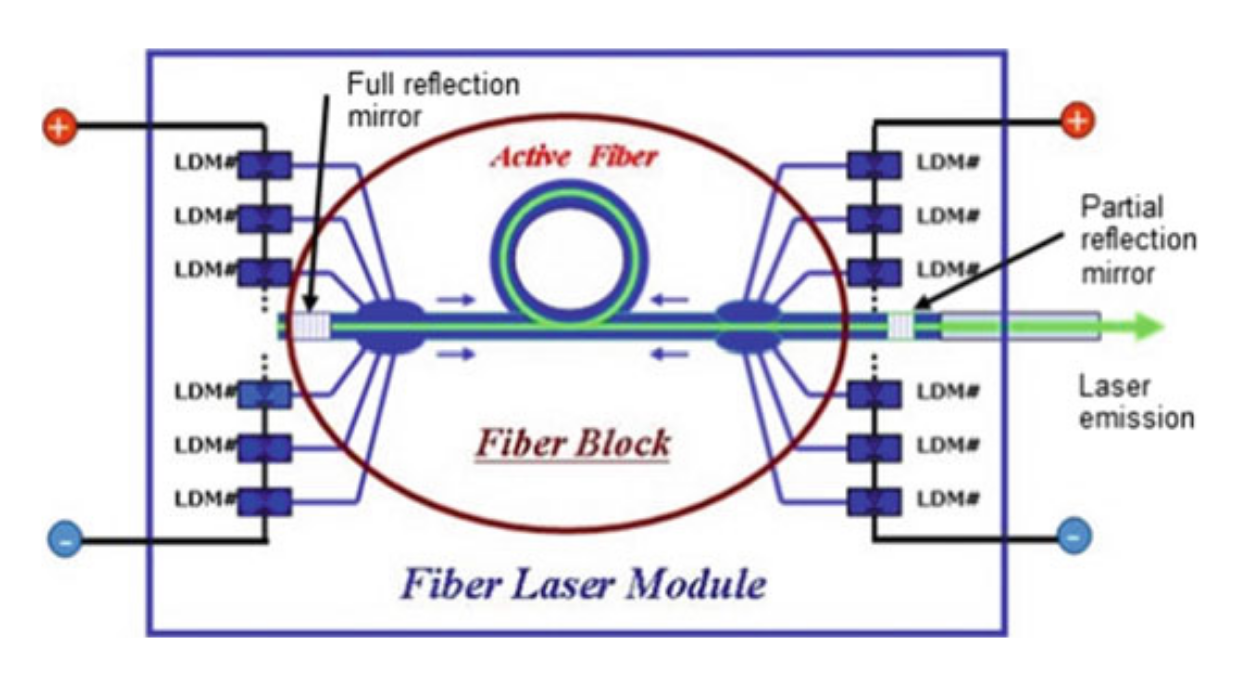
\includegraphics[scale=0.3]{Images/detailedfiber.png}}
    \caption[Laser diode and fiber laser.]{Emission mechanism of laser diode (a) and a detailed fiber laser schema (b) \cite{katayama_fundamentals_2020}.}
\end{figure}
In fiber lasers, the beam is emitted by an LD pumping and a fiber of high purity \ce{SiO2} quartz glass doped with \ce{Yb^3+} rare earth element. The diameter of the fiber is about \numrange[range-phrase=--]{10}{20}\unit{\micro\metre}. In this laser technology, optical pump diodes are coupled to an active laser fiber that has a unique reflective coating and two Bragg gratings that reflect the laser light back and forth along the length of the fiber to create a coherent beam of light at the output of the laser \cite{milewski_additive_2017}. Fig. \ref{fig:detailedfiber} shows full reflection mirror and partial reflection mirror installed next to the fiber. This also means that the laser beam adjustment is unnecessary, which means easier system handling. Combining multiple laser modules using a beam combiner for a more powerful laser is also possible. We can use additional optical fibers to deliver and contain the light energy, providing a robust, flexible, and fully enclosed beam path for beam delivery \cite{milewski_additive_2017}. Fiber laser has many advantages, such as high beam quality, the fact they are small and lightweight, high intensity (which allows higher scan speed) and high efficiency (cost decreasing), long-distance delivery, and require no maintenance. 
\subsection{Electrons-Matter Interaction}
\label{subsec:ebminter}
According to \citeauthor{schultz_h_electron_1994} (1994), while the physical characterization of electrons has been recognized since the 1960s, the microscopic processes still need a comprehensive quantitative explanation nowadays. However, a comprehensive explanation of electrons properties and their interaction with matter was given by \citeauthor{krumeich_properties_2015} (2015).
\subsubsection{What is an Electron?}
\label{sssec:electron}
An electron is a fundamental subatomic particle that carries a negative electric charge and is one of the primary constituents of atoms. As explained in Section \ref{subsec:ebm}, the electron beam is made of electrons generated through the thermionic effect with a metallic filament. An accelerating voltage $V$ is applied at the cathode, causing electrons acceleration till velocity $v$. As explained in \citeauthor{krumeich_properties_2015} (2015), we can write the equation for kinetic energy associated with an electron as 
\begin{equation}
    \label{eq:energyelectron}
    E  = e\cdot V = \frac{1}{2}mv^2
\end{equation}
Given the fact that electron mass is \SI{9.109e-31}{\kilo\gram}, electron charge is \SI{-1.602e-19}{\coulomb} and that a common voltage for EBM application is \SI{60}{\kilo\volt}, from \ref{eq:energyelectron} we find that electron velocity is
\begin{equation}
\label{eq:velocityelectron}
v=\frac{\sqrt{2\cdot e\cdot V}}{m}
\end{equation}
which is approximately \num{1.453e8} \unit{m/s} (about half the speed of light). Recalling the dualism wave-particle of the electron, we can use the De Broglie equation to compute the wavelength of the electron beam \cite{krumeich_properties_2015}:
\begin{equation}
\label{eq:wavelength}
    \lambda = \frac{h}{\sqrt{2\cdot m \cdot e \cdot V}}
\end{equation}
where $h=$\SI{6.62607015e-34}{\joule.\second} is the Planck constant. In case of a voltage higher than \SI{300}{\kilo\volt}, it is necessary to include a term that accounts for the relativistic nature of mass in \ref{eq:wavelength}, as the electron's speed would approach the speed of light.
\subsubsection{Magnetic Lenses in EBM}
\label{sssec:magneticlens}
In EBM, electromagnetic lenses control the beam's characteristics. As the beam passes through these lenses, the astigmatic lens adjusts the shape of the electron beam spot, the focus coil changes the spot size, and the deflection coil moves the beam along the x and y axes.
\begin{figure}
    \centering
    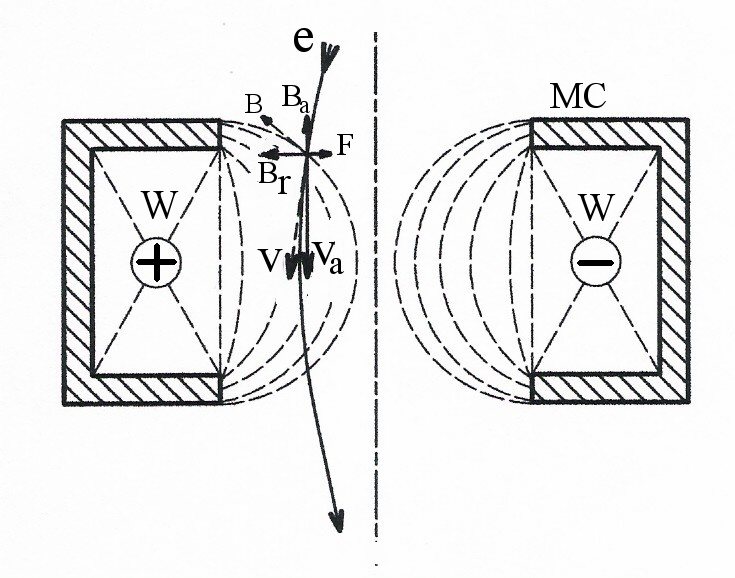
\includegraphics[scale=0.8]{Images/Magnetic_lens.jpg}
    \caption[Magnetic lens.]{Forces schema when an electron passes through magnetic lens \cite{wikipedia_magnetic_2023}.}
    \label{fig:magneticlens}
\end{figure}
The force $\mathbf{F}$ which an electron of charge $-e$ experiences when traveling with a velocity $\mathbf{v}$ due to a magnetic field $\mathbf{B}$ is given by Lorentz's law:
\begin{equation}
    \mathbf{F} = -e\cdot \left( \mathbf{v} \times \mathbf{B}\right)
\end{equation}
We can decompose the magnetic field into a radial component $\mathbf{B}_R$ and an axial component $\mathbf{B}_L$. The initial direction of the electron is parallel to the axis. Thus, it is only subjected to the radial component $\mathbf{B}_R$, responsible for a force orthogonal to $\mathbf{v}$. Hence, electrons start rotating. When they start spinning, they are subject to the axial field of the magnetic field, too, which results in a reducing radius spiraling trajectory that converges towards the targeted point.

\subsubsection{Electrons Interaction}
\label{sssec:electroninteractions}
As explained in \citeauthor{korner_additive_2016} (2016), we can distinguish two interaction types between electrons and matters, defined according to transferred energy quantity. 
\paragraph{Elastic interactions.} The electron's energy remains constant: when electrons penetrate the surface, they engage as negatively charged particles with the metal's negative field and the positive charge from the nucleus's protons. Electrons can be rerouted on a different path without losing kinetic energy (known as elastic scattering). After several interactions, deflected electrons sometimes exit from the metal. This phenomenon is called backscattering. This event occurs because of the Coulomb interaction, which happens when a negatively charged entity (electron) comes close to a positively charged one (nucleus). The equation describes Coulomb force:
\begin{equation}
    \label{eq:coulomb}
    F=\frac{Q_1\cdot Q_2}{4\pi \varepsilon_0 r^2}
\end{equation}
where $r$ is the distance between the charges $Q_1$ and $Q_2$ and $\varepsilon_0=$ \SI{8.854e-12}{\farad / \metre} is the dielectric constant. The backscatter phenomenon is determined by material characteristics and the angle at which the beam hits the metal surface; see Fig. \ref{fig:backscattering}. The phenomenon represents an energy deduction from the melting procedure. Indeed, if an electron exits the material, it cannot transfer energy to the material itself. So, for process efficiency, we have to avoid these interactions. The backscattering effect probability is directly proportional to the atomic number $Z$ of the material of the powder, specifically to $Z^2$.
\begin{figure}
    \centering
    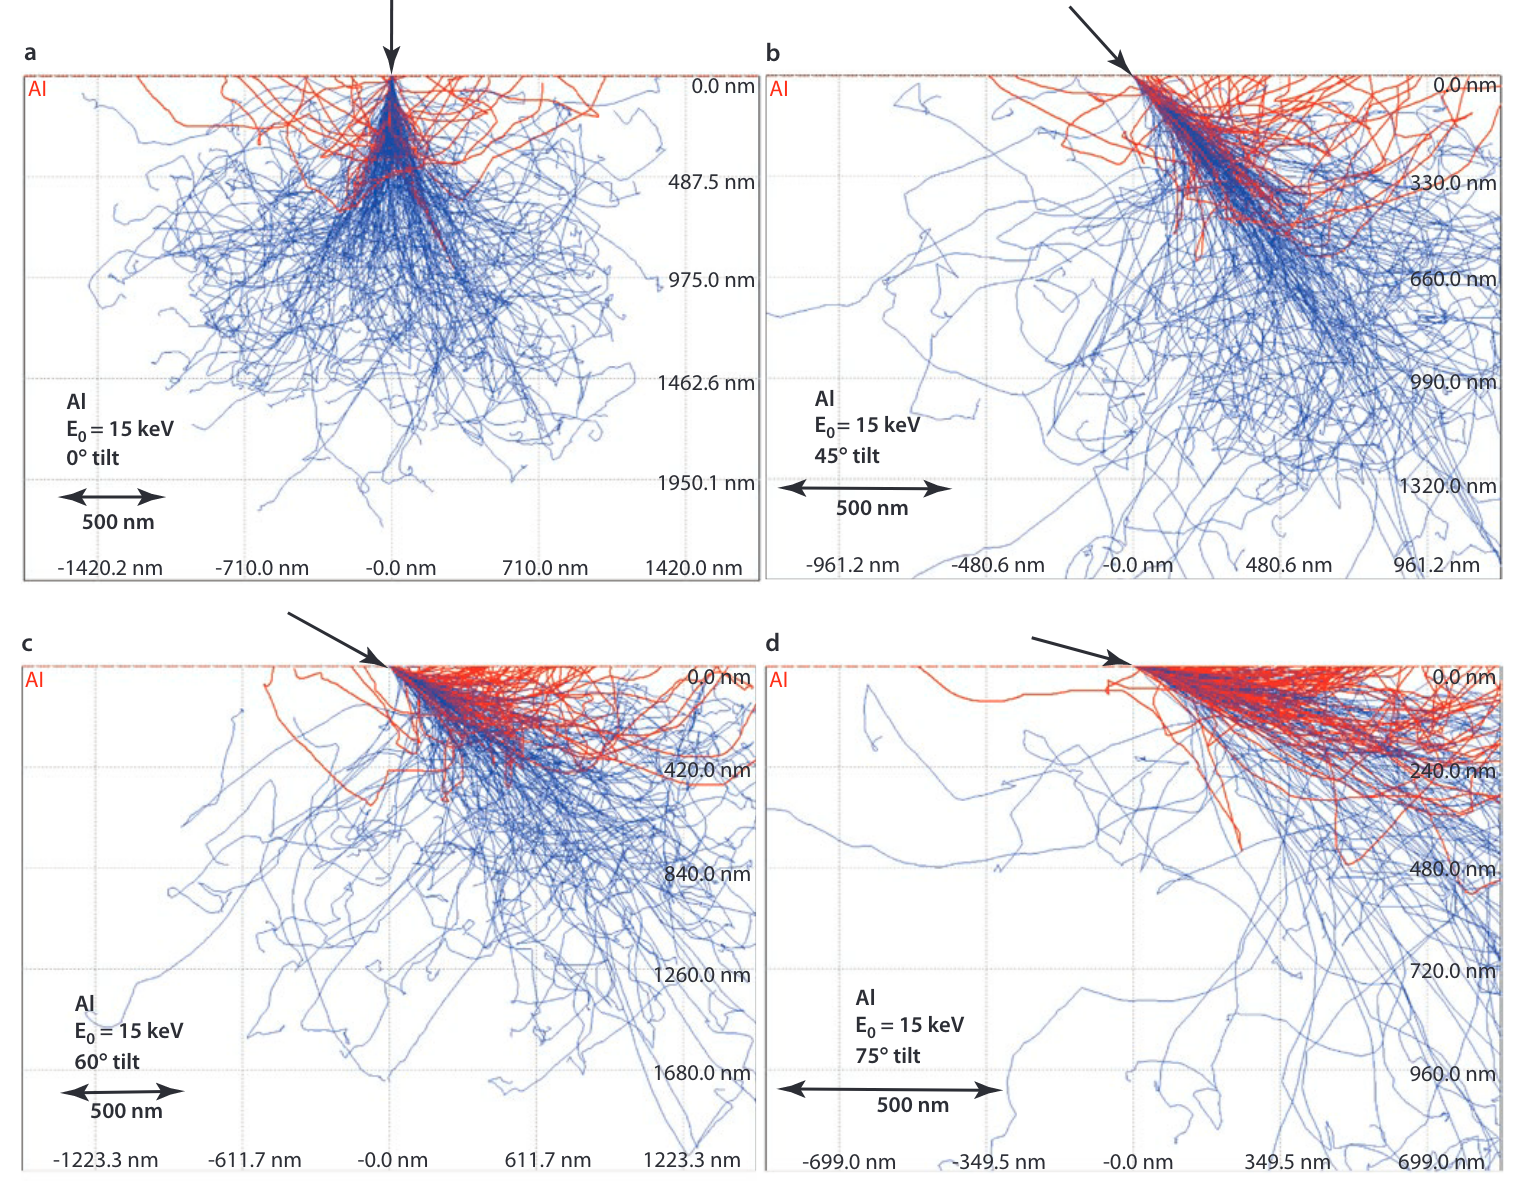
\includegraphics[scale=0.35]{Images/backscattering.png}
    \caption[Backscattering of an electron at different angles.]{Montecarlo simulation for an aluminum specimen hit by an electron beam at different angles, \ang{0}, \ang{45}, \ang{60}, \ang{75} respectively \cite{goldstein_scanning_2018}. In red, backscattered electrons.}
    \label{fig:backscattering}
\end{figure}
Moreover, the backscattering effect is increased when the electron beam hits the metal surface at highly inclined angles. A fine and as spherical as possible powder is essential to reduce the backscattering effect caused by the incidence angle. In EBM processes, the more spherical the particles are, the more we can assume that the electron beam will strike the particle surface perpendicularly. We can see in Fig. \ref{fig:particles} why.
\paragraph{Inelastic Interactions.} In inelastic interactions, the energy of the electrons diminishes. The energy released to the sample results in the heating of the metal and its corresponding melting. These interactions cause the release of certain emissions, detailed below \cite{krumeich_properties_2015, goldstein_scanning_2018}.
\begin{itemize}
    \item \textbf{Inner-shell ionization :} the energy is passed to an inner electron, which ejects it from the atom. This results in an unstable atom configuration, leading to the release of X-rays or an Auger electron. X-rays are produced when an inner electron is released into the vacuum, and an electron from the valence shell descends to occupy the void left by the electron from a deeper level. On the other hand, an Auger electron is produced when the core electron, stimulated by the electron beam's energy, is expelled into the vacuum. Another electron from a higher level occupies the left space, which then radiates energy to a closer electron until it is released into the chamber. That is why, in an EBM 3D printer, it is crucial to have a shield to protect operators from X-rays.
    \item \textbf{Braking radiation:} the electron that enters the atom slows down due to its interaction with the positively charged nucleus. The subsequent reduction in energy is released as X-rays. The material completely absorbs X-rays of lower energy, while X-rays of higher energy are released in the printing chamber.
    \item \textbf{Secondary electron:} Electrons within the valence band require minimal energy to surpass the potential barrier, and various electron-matter interaction mechanisms can provide this energy. This can cause the release of these electrons in the printing chamber. The inert gas flow in the chamber removes these electrons from the powder bed since they can interfere with the printing process.
    \item \textbf{Cathodoluminescence:} when an electron from the valence band rises to the conduction band, a vacancy is created in the valence band. Another electron descending from the conduction band occupies this vacancy, which releases a photon. This phenomenon is responsible for the characteristic light produced when the electron beam hits the metal powder in EBM. 
    \item \textbf{Plasmon:} an electron moving through the collection of electrons in the valence band can cause a disturbance, leading to a collective vibration of the free electrons. This interaction is prevalent in metals but can also occur in any substance with free electrons. This phenomenon is responsible for the creation of plasma oscillation.
    \item \textbf{Phonons:} Phonons are understood as the collective oscillations of atoms within a crystal lattice, resulting from inelastic engagements with the electron beam. When an atom initiates this vibrational movement, it conveys this activity throughout the lattice, impacting a significant volume. Phonons are the only ones responsible for the melting of metal powders. Other products are undesirable or even accountable for side effects during the printing process.
\end{itemize}
\begin{figure}
    \centering
    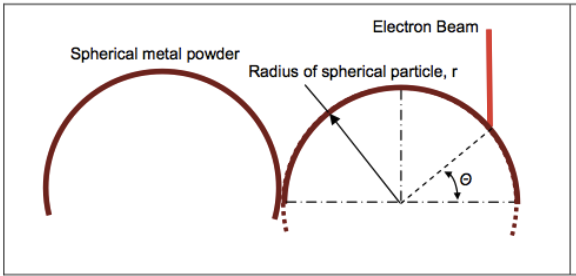
\includegraphics[scale=0.7]{Images/EBMparticles.png}
    \caption[Laser interactions and laser intensity.]{Electron beam interaction with spherical powder particles (a) \cite{tushar_ramkrishna_mahale_electron_2009}.}
    \label{fig:particles}
\end{figure}
% <<< End of Energy Matter Interactions

%%%%%
%%%%%

% Applications of PBF Metal Additive Manufacturing >>>
\section{Applications of PBF Metal Additive Manufacturing}
\label{sec:examplesPBF}
One of the primary advantages of PBF processes is the capability to produce finished objects unattainable with traditional manufacturing systems. This section presents some examples of how this technology can completely disrupt the production processes of metal components manufacturing. The nozzle in Fig \ref{fig:nozzle} is one of the most famous, successful, and documented examples of metal AM. General Electrics designed it in 2015. Using AM, GE could produce the nozzle in a single piece rather than 20 pieces welded together. They were able to reduce weight by 25\%, which was five times more durable and 30\% more cost-efficient \cite{amy_kover_transformation_2018}. GE Aviation has set the goal of 32,000 nozzles per year in whole production \cite{milewski_additive_2017}, opening this process to large-scale distribution. In 2015, NASA designed the first 3D-printed rocket nozzle made of copper. Within the combustion chamber, the propellant burns at temperatures exceeding \SI{3000}{\kelvin}. Hydrogen at temperatures just above \SI{100}{\kelvin} flows through over 200 intricately designed cooling channels to prevent it from melting. Fig. \ref{fig:nozzlerocket} shows cooling inlets integrated into the chamber's top rim. Thanks to this rocket nozzle, costs were reduced by 50\%, and manufacturing times were reduced by ten times \cite{tracy_mcmahan_nasa_2015}, opening the path to a more affordable and lean space industry. Fig. \ref{fig:piston} shows Porsche's application of PBF processes in the automotive sector. The company managed to print pistons by PBF for the 911 GT2 RS engine. These new pistons have achieved a temperature on the piston's o-ring that is \SI{20}{\degreeCelsius} lower than usual. This leads to an additional \SI{23}{\kilo\watt} power available. However, we will have to wait until at least 2030 before we see large-scale production, according to Porsche's press release \cite{roberto_baldwin_porsches_2020}. AM is also being employed in the medical field, for example, in dentistry. Custom-fitted designs are transforming the traditional ways of fabricating items like crowns and dental implants. Advanced high-precision 3D printers, such as EOS M 100 DMLS, can print devices from Cobalt Chrome SP2 alloy, a medical-grade approved material in the medical field \cite{milewski_additive_2017}. Products with small batch sizes, high precision, and significant value, like these dental devices, are increasingly manufactured using these new technologies. The advantages of AM include the swift creation of tailor-made items for immediate application, such as implants, or indirect uses like drill guides and fixtures, all based on the patient's medical characteristics for a perfect fit. Moreover, the surface finish or porous structures offer better support for bone growth. In Fig. \ref{fig:skul}, there is an example of a titanium skull implant.
\begin{figure}
    \centering
    
    \subfloat[\label{fig:nozzle}]{
        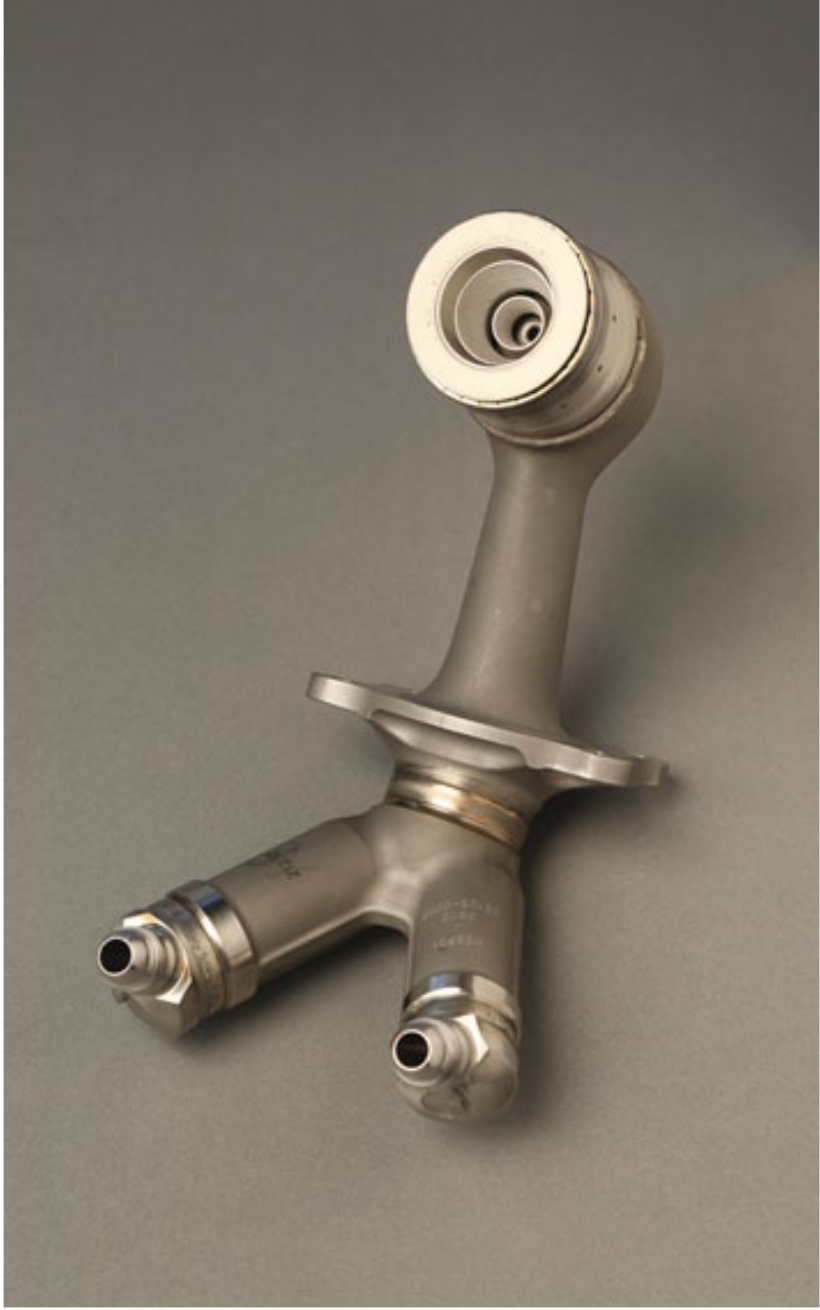
\includegraphics[scale=0.20]{Images/nozzle.png}
    }
    \qquad
     \subfloat[\label{fig:nozzlerocket}]{
        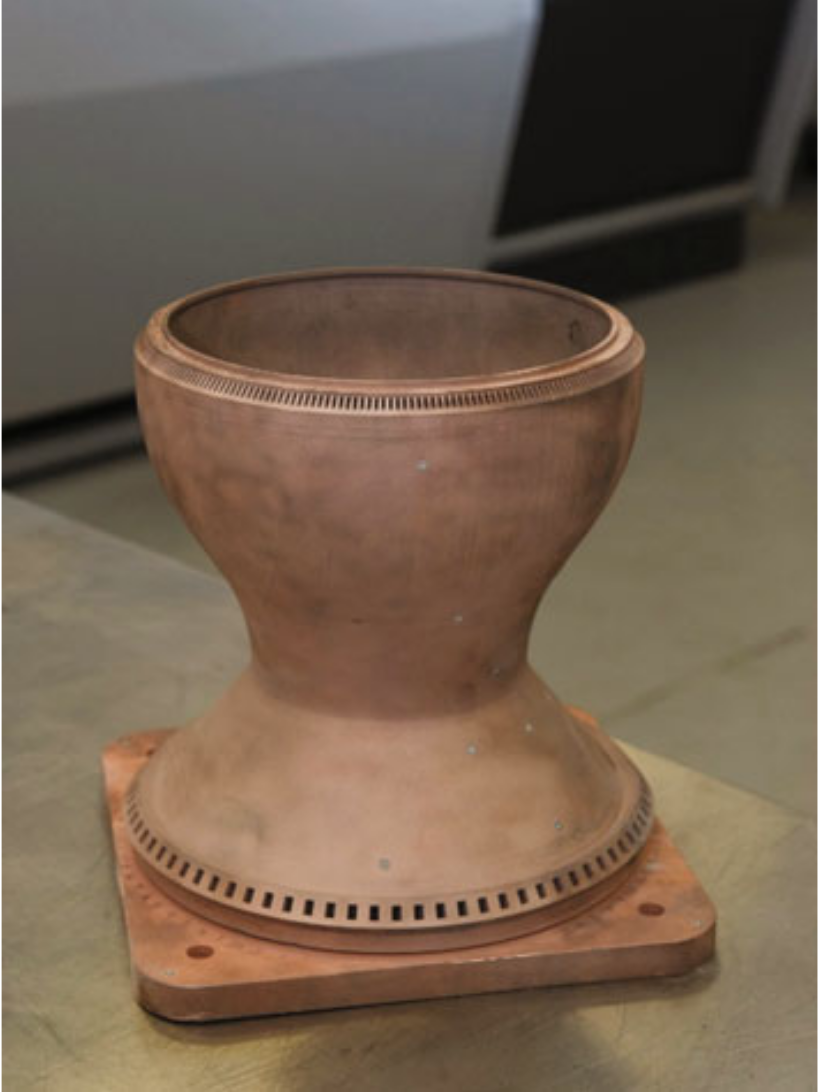
\includegraphics[scale=0.24]{Images/nozzlerocket.png}
    }
    \\
    \subfloat[\label{fig:piston}]{
        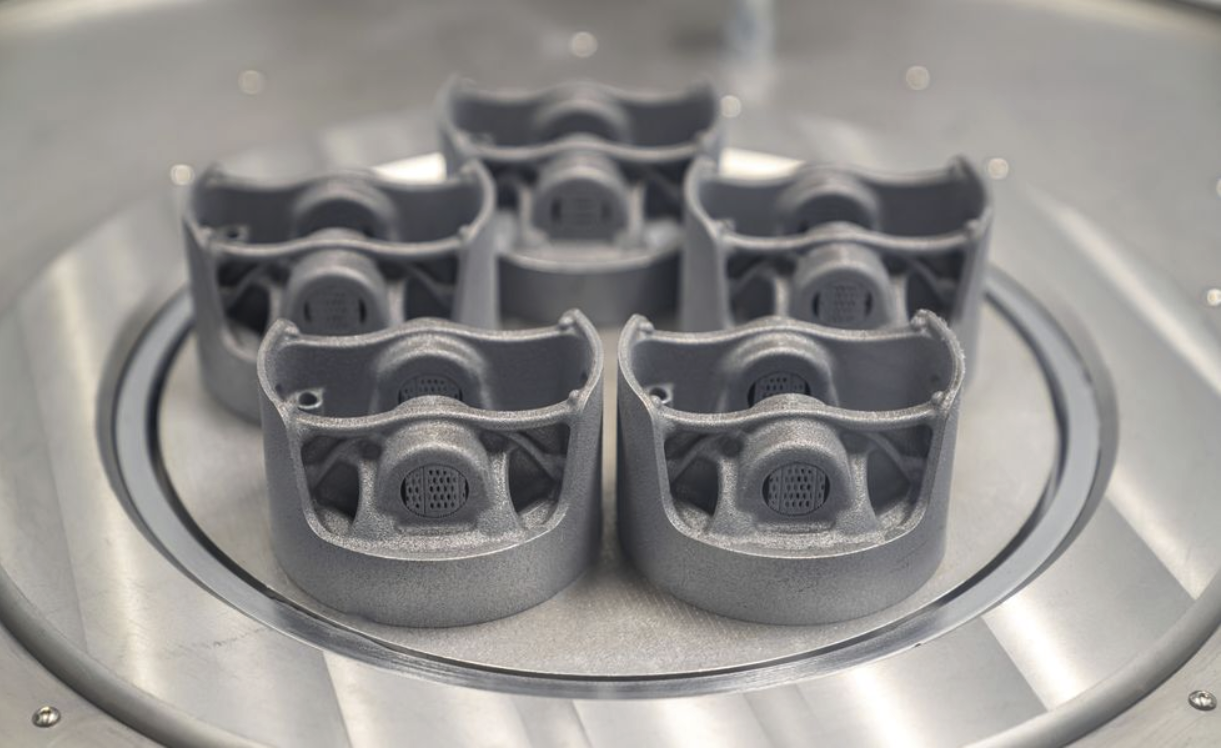
\includegraphics[scale=0.21]{Images/piston.png}
    }
    \qquad
    \subfloat[\label{fig:skul}]{
        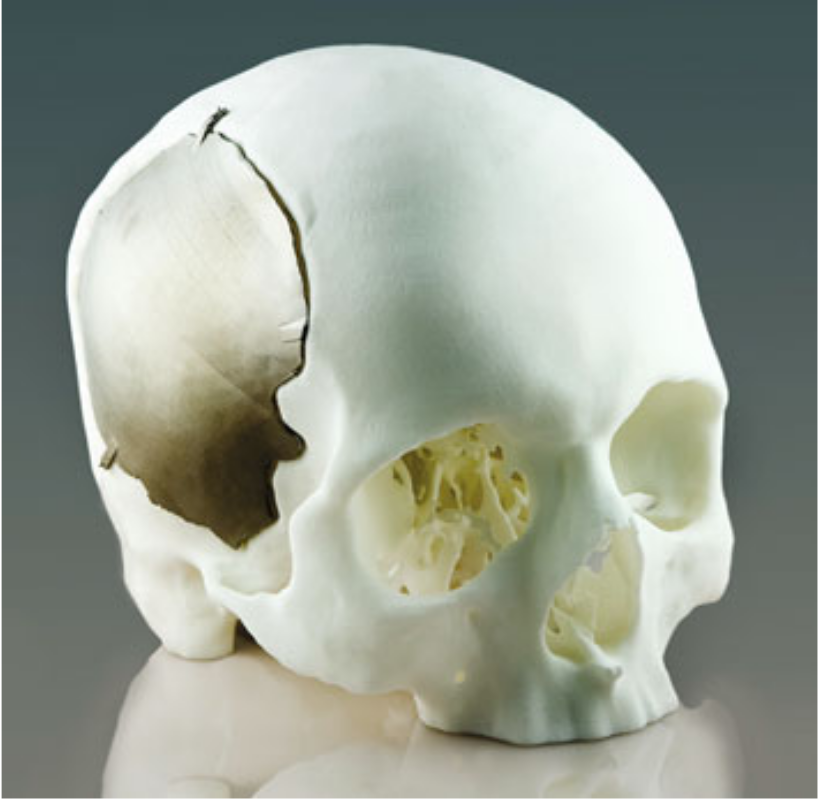
\includegraphics[scale=0.20]{Images/skull.png}
    }
    
    \caption[Examples of metals AM.]{Examples of metal AM: GE nozzle used in airplane turbines to mix fuel and air (a), a rocket nozzle in copper by NASA (b), Porsche engine pistons (c), and a titanium skull implant (d).}
    \label{fig:amexamples}
\end{figure}

\subsection{Lattice Structure and Cellular Material} \label{subsec:lattice}
A specific application of PBF processes is the production of so-called lattice structures. In recent years, biomimicry techniques have spread in additive manufacturing. Biomimicry is a set of design techniques that allow us to take inspiration from nature to find solutions to engineering problems or to design functional components that can be used in engineering applications \cite{pathak_biomimicry_2019, du_plessis_beautiful_2019}. Over the past 3.8 billion years, nature has found the most efficient way to develop functional solutions to evolutionary problems characterized by immovable constraints. Moreover, during the evolutionary process of species, nature has created nano, micro, and macro-structures that provide unique structural properties, adapting shape to function and using the bare minimum to achieve the evolutionary goal. Indeed, one of life's principles explained in \citeauthor{baumeister_biomimicry_2011} (2011) states \textit{"Life integrates and optimizes these strategies to create conditions conducive to life"}. Therefore, biomimicry consists in creating new multi-functional structures with unique characteristics, optimizing materials, and reducing waste. Engineers have always been fascinated by cellular materials, evident from the first reference to the idea that structure could influence a material's functional characteristics and behavior, which Robert Hooke made in 1665 \cite{l_gibson_cellular_2010}. Thanks to the computational power of CAD software, only in recent years has it been possible to experiment with the mechanical characteristics of 3D-printed lattice structures. Lattice structures are such an example of bio-inspired designs. According to ISO/ASTM, 52900 \cite{organization_isoastm_2015}, \emph{lattice structure} are "three-dimensional geometric arrangement composed of connective links between vertices (points) creating a functional structure". Lattice structures are three-dimensional structures made up of different connected single elements called "cells" that can have different shapes designed to meet the desired mechanical features of the final object. These objects are distinguished by empty spaces within the structure and can only be obtained thanks to layer-wise AM technologies. 
As example, an aluminum cube formed from dodecahedron-shaped cells printed using only \SI{3.9}{g} of material and can support a weight of \SI{408}{Kg}, which means it can withstand a stress of 100,000 times its weight \cite{noauthor_3d_2014}. 
\begin{figure}
    \centering
    \subfloat[\label{fig:heatexchanger}]{
        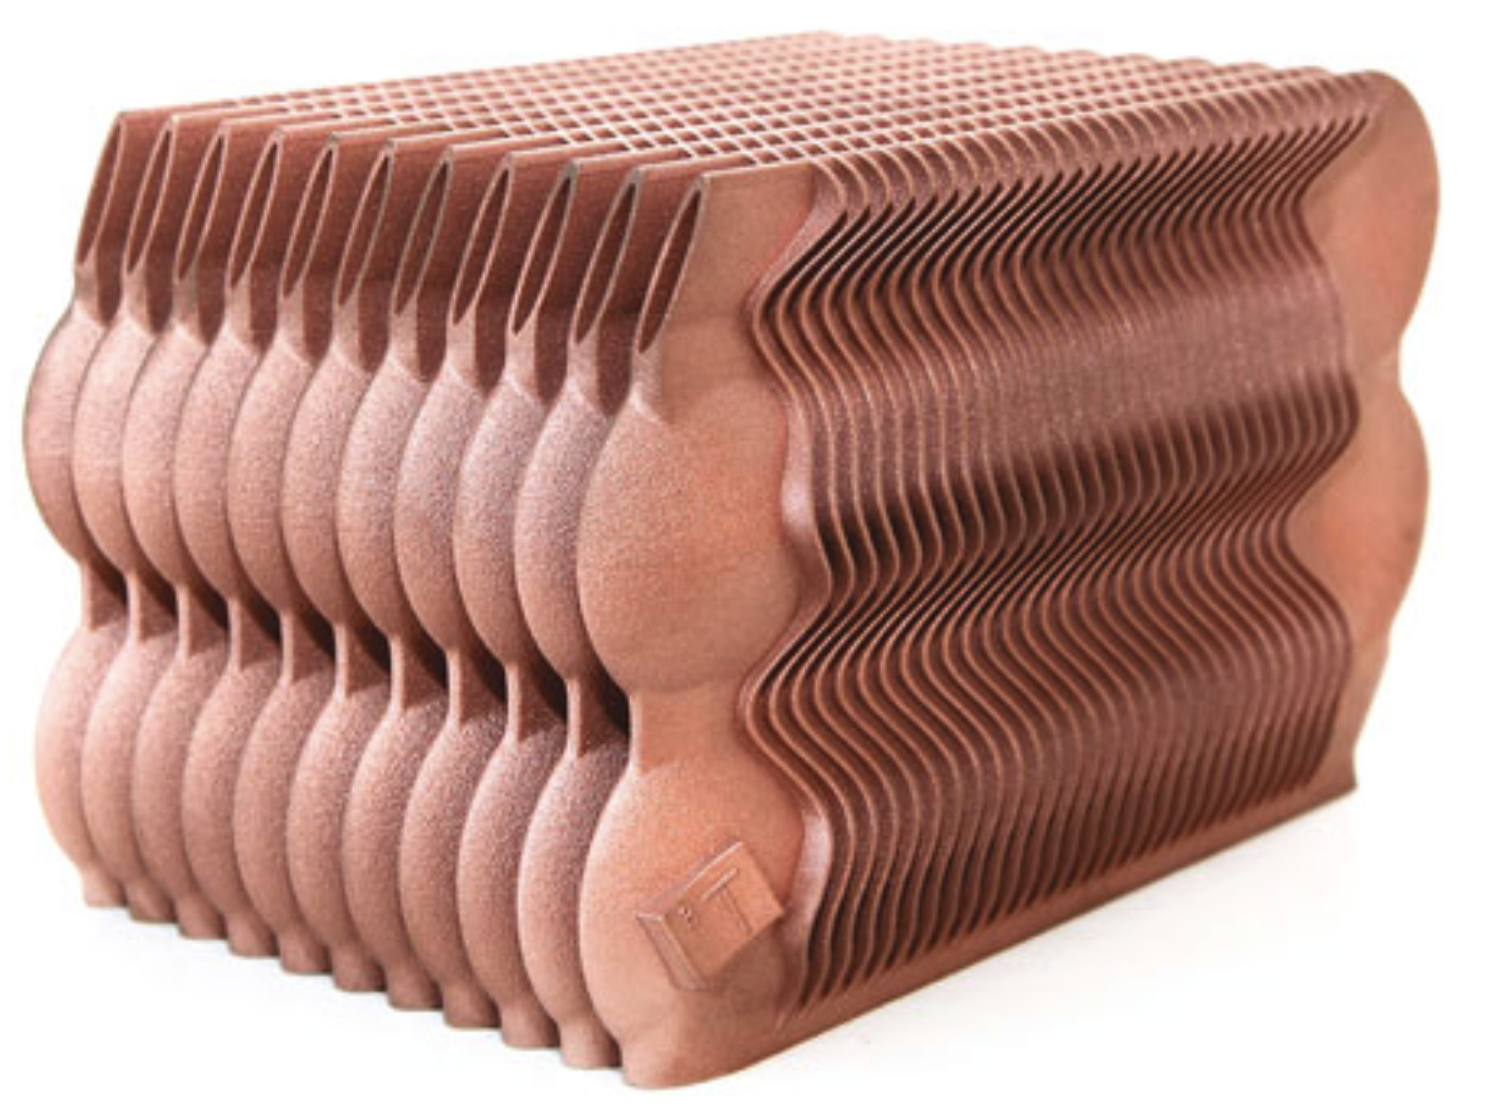
\includegraphics[width = 0.35\textwidth]{Images/heatexchanger.png}
    }
    \qquad
    \subfloat[\label{fig:f1freno}]{
        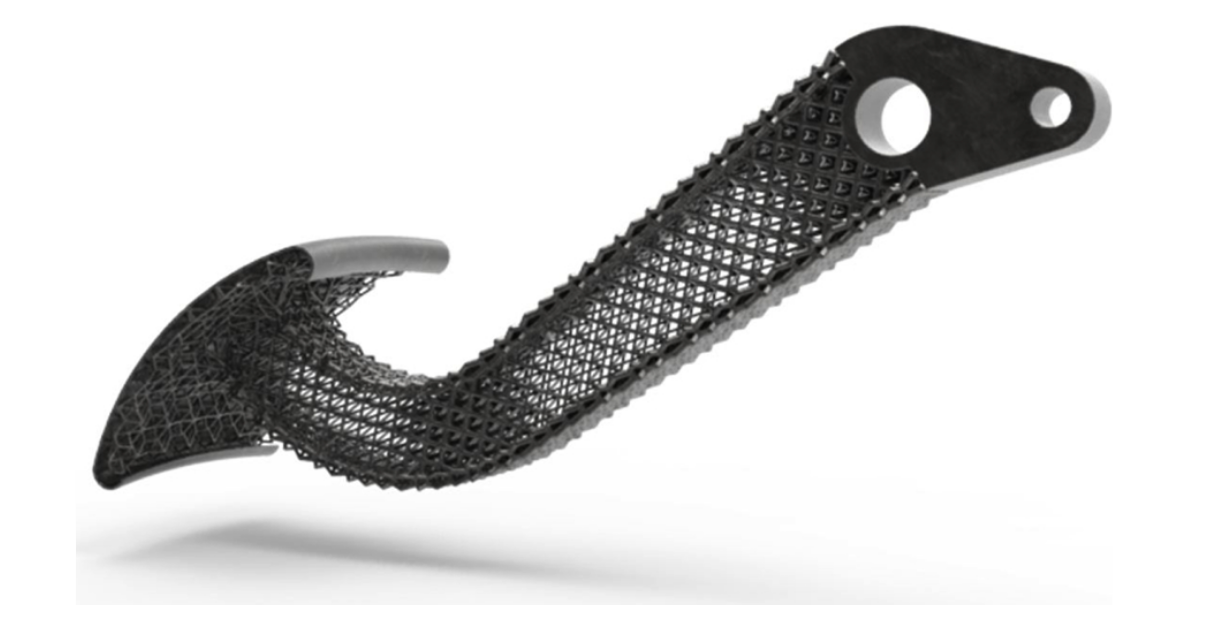
\includegraphics[width = 0.35\textwidth]{Images/f1freno.png}
    }
    \caption[Lattice structure applications.]{Examples of lattice structure application: a complex heat exchanger (a) and brake pedal of F1 racing car (b) \cite{milewski_additive_2017, du_plessis_beautiful_2019}}.
\end{figure}
Lattice structures can be used as space-filling structures, as an improvement to surface structures' strength and resilience, and to reduce the weight of the printed component. These versatile structures can be effectively applied in various engineering fields to address multiple challenges. Specifically, they are commonly used in four main areas according to \citeauthor{bhate_classification_2019} (2019): 
\begin{itemize}
    \item \textbf{Structural engineering} for vibration control, strain isolation, and weight reduction purposes like in Fig. \ref{fig:f1freno};
    \item \textbf{Thermal engineering} for applications such as heat exchangers in Fig. \ref{fig:heatexchanger}, flame arresters, or heat shields;
    \item \textbf{Fluid dynamics engineering} which employs lattice structures as catalyst carriers or packaging;
    \item \textbf{Biomedical engineering}, where lattice structure can be leveraged for bone integration in prosthetic and cell growth
\end{itemize}
% <<< End of Applications of PBF Metal Additive Manufacturing